\documentclass[10pt, aspectratio=169,t,xcolor=table]{beamer}

\setlength{\itemsep}{0pt}
\setlength{\parskip}{0pt}
\setlength{\parsep}{0pt}

\usetheme{Finalyear}

\usepackage{multicol}
\usepackage{pdfpages}
\usepackage{appendixnumberbeamer}
\usepackage{tabularx}
\usepackage{adjustbox}
\usepackage{enumitem}
% \setlist{nosep, leftmargin=*}
\newcommand{\shadowsq}{%
    
\begin{tikzpicture}
        \fill[gray!90] (0.02,-0.05) rectangle (0.12,0.05);
        \fill[black] (-0.02,-0.02) rectangle (0.08,0.08);
        % \draw[white, very thin] (0,0.25) -- (0,0) -- (0.25,0);
    \end{tikzpicture}%
}
\setlist{label=\shadowsq, itemsep=0.1pt, parsep=1pt, topsep=5pt, leftmargin=8pt}
\usepackage{fontawesome5}
\usepackage[
    style=authoryear,
    backend=biber,
    language=english,
    dashed=false
]{biblatex}
\AtBeginBibliography{\footnotesize}
\addbibresource{references.bib}
\setbeamertemplate{bibliography entry title}{}
\setbeamertemplate{bibliography entry location}{}
\setbeamertemplate{bibliography entry note}{}
\setbeamercolor{bibliography item}{fg=blue!80}
\setbeamercolor{bibliography entry author}{fg=black}
\setbeamercolor{bibliography entry title}{fg=black}

\setbeamertemplate{bibliography item}[triangle] % icons
\setbeamercolor{cite}{fg=red!10!black}
\DeclareCiteCommand{\cite}[\mkbibbrackets]
  {\usebibmacro{prenote}}%
  {\usebibmacro{citeindex}%
    \printtext[bibhyperref]{\tiny \textbf{\printnames{labelname}, \printfield{year}}}}%
  {\multicitedelim}%
  {\usebibmacro{postnote}}%

\ExecuteBibliographyOptions{dashed=false}

\setbeamerfont{frametitle}{size=\fontsize{11}{11}\selectfont}
\setbeamercolor{bibliography item}{fg=black!80}
\setbeamercolor{footnote mark}{fg=blue!80}

% Open refrence from local dir
% \newcommand{\pdflink}[2]{\href{../papers/#1.pdf}{#2}}
% \newcommand{\pdflink}[2]{\href{run:../papers/#1.pdf}{#2}}
\newcommand{\pdflink}[2]{\href{file:papers/#1.pdf}{#2}}

\setbeamercolor{cite}{fg=red!10!black}
\DeclareCiteCommand{\cite}[\mkbibbrackets]
  {\usebibmacro{prenote}}%
  {\usebibmacro{citeindex}%
    \printtext[bibhyperref]{\tiny \textbf{\printnames{labelname}, \printfield{year}}}}%
  {\multicitedelim}%
  {\usebibmacro{postnote}}%

\ExecuteBibliographyOptions{dashed=false}

\definecolor{darkgreen}{RGB}{0,100,0}
\definecolor{darkred}{RGB}{139,0,0}

% Theorem environments
\newtheorem{conj}{Conjecture}
\newtheorem{defi}{Definition}
\newtheorem{teo}{Theorem}

\setbeamertemplate{theorems}[numbered]
\setbeamertemplate{caption}[numbered]
\setcounter{figure}{0}

\setPrimaryColor{MyBlue}
\setLogos{lib/logo/iist-logo-horizontal.png}{lib/logo/iist-logo-square.png}

\begin{document}
% -------------------------------------------------------------------
%  TITLE INFORMATION
\title[MD Land-Atmosphere Coupling]{Land-Atmosphere Coupling in Monsoon Depressions via Soil Moisture Feedback}
\subtitle{Impact of Land-Surface Feedback on Post-Landfall Sustainability of Monsoon Depressions}
\author{}
\date{}
% \author[Harshit P. D.]{
% 	\begin{columns}
% 		\column{0.4\textwidth}
% 		\centering
% 		\textbf{Presented by:} \\
% 		\textbf{Harshit Prashant Dhanwalkar} \\
% 		\tiny{SC21B164} \\
% 		\tiny{Earth System Sciences (ESS)}
%
% 		\column{0.4\textwidth}
% 		\centering
% 		\textbf{Supervisor:} \\
% 		Dr.\ A.\ Chandrasekar
% 	\end{columns}
% 	\hfill
% }
\setbeamertemplate{title page}{
	\vfill
	\begin{centering}
		\usebeamerfont{title}\usebeamercolor[fg]{title}\inserttitle\par
		\vspace{0.2cm}
		\usebeamerfont{subtitle}\usebeamercolor[fg]{subtitle}\insertsubtitle\par
		\vspace{0.5cm}

		\begin{columns}[T]
			\column{0.45\textwidth}
			\centering
			\textbf{Presented by:} \\
			\textbf{Harshit Prashant Dhanwalkar} \\
			\tiny{SC21B164} \\
			\tiny{Earth System Sciences (ESS)}

			\column{0.45\textwidth}
			\centering
			\textbf{Supervisor:} \\
			Dr.\ A.\ Chandrasekar
		\end{columns}
		\vfill
	\end{centering}
}
\frame[noframenumbering]{\titlepage}

% -------------------------------------------------------------------
%  TABLE OF CONTENTS
% \setLayout{plain}
% \begin{frame}[plain, c]{Table of Contents}
% 	\vspace{-0.3cm}
% 	\setbeamerfont{section in toc}{size=\fontsize{7}{8}\selectfont}
% 	\setbeamerfont{subsection in toc}{size=\fontsize{5.5}{6.5}\selectfont}
% 	\setbeamertemplate{section in toc}[sections numbered]
% 	\setbeamertemplate{subsection in toc}{\leavevmode\leftskip=0.6em\inserttocsubsection\par}
% 	\begin{multicols}{3}
% 		\tableofcontents
% 	\end{multicols}
% \end{frame}

% -------------------------------------------------------------------
\section{Introduction}
\setLayout{mainpoint}
\begin{frame}{}
	\frametitle{INTRODUCTION}
\end{frame}

% -------------------------------------------------------------------
\setLayout{vertical}
\begin{frame}{Monsoon Depression Inland Longevity}
	\footnotesize
	\begin{itemize}
		\item \textbf{Monsoon Depressions (MDs):} Large, slow-moving low-pressure systems
		      forming over the Bay of Bengal that are responsible for $\mathbf{>50\%}$ of
		      total Indian monsoon rainfall, with a typical lifespan of $\sim$2–7 days.
		      \vspace{0.25cm}
		\item \textbf{The Longevity Paradox:} Some MDs decay within 3 days of landfall.
		      Others persist for 7+ days deep inland - far from any oceanic moisture source.
		      What drives this difference?
		      \vspace{0.25cm}
		\item \textbf{The Brown Ocean Hypothesis:} Wet, clay-rich soils of the
		      Indo-Gangetic Plain mimic the ocean's latent heat supply - providing a
		      \textit{secondary energy source} that can sustain an MD long after it
		      leaves the Bay of Bengal.
		      \vspace{0.25cm}
		\item \textbf{Research Gap:} Despite well-studied atmospheric dynamics, the
		      \textit{quantitative role of land-atmosphere coupling} - specifically
		      soil moisture $\leftrightarrow$ precipitation feedback - remains poorly
		      constrained in operational forecasting.
	\end{itemize}
	\vspace{0.2cm}
	\begin{alertblock}{\small Practical Significance}
		\scriptsize
		Duration directly determines total rainfall, flood potential, and forecast skill.
		Current models have useful skill only to $\sim$72–96 h post-landfall.
		Land-surface factors are systematically underrepresented.
	\end{alertblock}
\end{frame}

% -------------------------------------------------------------------
\setLayout{horizontal}
\begin{frame}{The Brown Ocean Effect - Physical Mechanism}
	\begin{columns}
		\column{0.92\textwidth}
		% \vspace{-0.3cm}
		\begin{block}{\small What is the Brown Ocean Effect?}
			\footnotesize
			Over inland, soils act as a \textbf{``pseudo-ocean''} energy reservoir:
			\begin{itemize}
				\item Volumatric Soil Water Layer (SWVL1) $\rightarrow$ enhanced evapotranspiration (ET)
				\item ET $\rightarrow$ large latent heat flux (LHF) to atmosphere
				\item LHF $\rightarrow$ increased atmospheric instability (CAPE)
				\item CAPE $\rightarrow$ deep convection \& precipitation feedback
				\item Total Precipitation (TP) $\rightarrow$ recharges soil moisture
			\end{itemize}
		\end{block}

		\vspace{0.2cm}
		\begin{block}{\small The Feedback}
			\centering
			\footnotesize
			\begin{tikzpicture}[
				node distance=1.5cm,
				box/.style={rectangle, draw, rounded corners=2pt, minimum width=1.2cm, minimum height=0.6cm, align=center},
				arrow/.style={-{Stealth[scale=1.2]}, thick}
				]
				\node[box] (tp) {TP};
				\node[box, right=of tp] (swvl1) {SWVL1};
				\node[box, right=of swvl1] (lhf) {LHF};

				\draw[arrow] (tp) -- node[above, font=\tiny] {recharge} (swvl1);
				\draw[arrow] (swvl1) -- node[above, font=\tiny] {ET} (lhf);
				\draw[arrow] (lhf.south) -- ++(0,-0.5) coordinate (corner)
				node[below, font=\tiny] at ($(lhf.south)!0.5!(corner)$) {}
				(corner) -- (corner -| tp.south) node[below, font=\tiny] at ($(corner)!0.5!(corner -| tp.south)$) {convection}
				(corner -| tp.south) -- (tp.south);
			\end{tikzpicture}
		\end{block}

		% \column{0.48\textwidth}
		% \vspace{-0.3cm}
		% \begin{block}{\small Key Metrics Developed}
		% 	\footnotesize
		% 	\begin{itemize}
		% 		\item \textbf{FSI} (Feedback Strength Index): TP–SWVL1 coupling strength
		% 		\item \textbf{CE} (Coupling Efficiency): How efficiently soil moisture
		% 		      is converted to sustained atmospheric heating
		% 		\item \textbf{ACF} (Autocorrelation at 24h): Soil moisture memory -
		% 		      does yesterday's wet soil persist today?
		% 		\item \textbf{TSI} (Topographic Sensitivity Index): Terrain's role in
		% 		      modulating feedback
		% 		\item \textbf{ASM} (Antecedent Soil Moisture): Pre-landfall soil state
		% 	\end{itemize}
		% \end{block}
	\end{columns}
\end{frame}

% % -------------------------------------------------------------------
% \setLayout{vertical}
% \begin{frame}{Research Objectives}
% 	\textbf{\small Primary Objective:}
% 	\footnotesize Quantify how land-surface conditions - soil moisture, soil type,
% 	terrain, and antecedent moisture - control post-landfall Monsoon Depression longevity.
%
% 	\vspace{0.3cm}
% 	\textbf{\small Six Testable Hypotheses:}
% 	\footnotesize
% 	\begin{enumerate}
% 		\item \textbf{H1 - Coupling Strength:} FSI $>$ 0.4 predicts long-lived MDs
% 		      ($\geq$96 h); FSI $<$ 0.1 predicts short-lived systems.
% 		\item \textbf{H2 - Diurnal Coupling:} Land-phase diurnal SHF amplitude
% 		      ($\sim$56 W/m$^2$) is $4\times$ stronger than ocean phase ($\sim$14 W/m$^2$).
% 		\item \textbf{H3 - Antecedent Moisture:} ASM strongly predicts FSI
% 		      ($r \approx 0.92$); wetter pre-monsoon soil $\to$ stronger coupling.
% 		\item \textbf{H4 - Landfall Transition:} Heat flux signature at landfall
% 		      distinguishes Ocean-to-Land from Land-origin tracks.
% 		\item \textbf{H5 - Soil Type:} Clay soils (IGP) sustain feedback; sandy coastal
% 		      soils break the loop via rapid runoff.
% 		\item \textbf{H6 - ASM Enables but Doesn't Ensure:} High ASM is necessary
% 		      but insufficient - requires clay texture, FSI $>$ 0.4, and ACF $>$ 0.3.
% 	\end{enumerate}
%
% 	\vspace{0.1cm}
% 	\begin{alertblock}{\small Null Hypothesis (H0)}
% 		\scriptsize
% 		Long-lived MDs show no systematic difference in TP–SWVL1 coupling,
% 		diurnal SHF, or soil memory compared to short-lived systems.
% 	\end{alertblock}
% \end{frame}
% -------------------------------------------------------------------

\section{Methodology}
% -------------------------------------------------------------------
\setLayout{mainpoint}
\begin{frame}{}
	\frametitle{METHODOLOGY}
\end{frame}

% -------------------------------------------------------------------
\setLayout{horizontal}
\begin{frame}{Dataset Information}
	\begin{columns}
		\column{0.8\textwidth}
		\begin{block}{\footnotesize ERA5 (ECMWF Reanalysis v5) Single Level Reanalysis Dataset\tiny \cite{hersbach2020era5}}
			\footnotesize
			\begin{itemize}
				\item \textbf{Source:} Copernicus Climate Data Store (CDS), ECMWF
				\item \textbf{Temporal Coverage:} June–September 2024 (4 months, Indian monsoon season)
				\item \textbf{Spatial Domain :} $10$--$30^\circ$ N, $70$--$95^\circ$ E (Indian subcontinent + Bay of Bengal)
				      % FIX: the spatial (31 km globally) and temporal (hourly) resolutions of ERA5
				\item \textbf{Resolution:} 0.25$^\circ$ $\times$ 0.25$^\circ$
				      ($\approx$27.75 km latitude $\times$ 24–28 km longitude over India)
				\item \textbf{Temporal frequency:} Hourly (1-hourly tracking)
				\item \textbf{Format:} NetCDF4; land-sea mask (LSM) applied for
				      ocean masking in analysis
			\end{itemize}
		\end{block}

		\column{0.2\textwidth}
		\begin{figure}
			\centering
			
\includegraphics[width=1\textwidth]{lib/logo/era5-logo.png}
		\end{figure}

		\vspace{0.2cm}
		\begin{figure}
			\centering
			
\includegraphics[width=1\textwidth]{lib/logo/Copernicus vecto def Europe's eyes on Earth.png}
		\end{figure}
	\end{columns}
\end{frame}

% -------------------------------------------------------------------
\setLayout{vertical}
\begin{frame}{Dataset Information}
	\vspace{-0.1cm}
	\begin{columns}[T]
		\column{0.44\textwidth}
		\begin{block}{\small ERA5 Dataset Variables :}
			\begin{itemize}\footnotesize
				\item Mean Sea Level Pressure (\texttt{MSL})
				\item Surface Pressure (\texttt{SP})
				\item 10-Meter U-Wind Component (\texttt{U10})
				\item 10-Meter V-Wind Component (\texttt{V10})
				\item Mean Surface Latent Heat Flux (\texttt{AVG\_SLHF})
				\item Mean surface Sensible Heat Flux (\texttt{AVG\_ISHF})
				\item Total Precipitation (\texttt{TP})
				\item Volumetric Soil Water Layer-1 (\texttt{SWVL1})
				\item Soil Temperature Level-1 (\texttt{STL1})
				\item 2-Meter Temperature (\texttt{T2M})
				\item 2-Meter Dew Point Temperature (\texttt{D2M})
			\end{itemize}
		\end{block}

		\column{0.55\textwidth}
		\begin{block}{\small Derived Variables :}
			\begin{itemize}\footnotesize
				\item \textbf{10-meter Wind Speed (\texttt{W10}) :}
				      \footnotesize
				      \begin{equation}
					      \texttt{W10} = \sqrt{(\texttt{U10})^2 + (\texttt{V10})^2}
				      \end{equation}
				\item \textbf{Relative Vorticity (\texttt{$\zeta$}):}
				      \footnotesize
				      \begin{equation}
					      \zeta = \frac{\partial(\texttt{V10)}}{\partial x} - \frac{\partial(\texttt{U10)}}{\partial y}
				      \end{equation}
				      % \item \textbf{Total Heat Flux (\texttt{THF}) :}
				      %       \footnotesize
				      %       \begin{equation}
				      % 	      \texttt{THF} = \texttt{SLHF} + \texttt{SSHF}
				      %       \end{equation}
				\item \textbf{Water Vapor Mixing Ratio (\texttt{w}) :}
				      \footnotesize
				      \begin{equation}
					      \texttt{w} = 0.622 \frac{e_s}{\texttt{SP} - e_s} \times 1000
				      \end{equation}
				      Where \textbf{Saturation Vapor Pressure (\texttt{$e_s$}) :}
				      \footnotesize
				      \begin{equation}
					      e_s = 6.112 \exp\left(\frac{17.67 * \texttt{D2M}}{\texttt{D2M} + 243.5}\right)
				      \end{equation}
				      and \texttt{D2M} = 2m Dew Point Temperature in $^\circ$C
			\end{itemize}
		\end{block}
	\end{columns}
	% \item \textbf{Processing :} Multi-month concatenation, temporal regularization, spatial clipping
\end{frame}

\begin{frame}{ERA5 Reanalysis Dataset Variables Selection}
	\begin{columns}
		\column{0.8\textwidth}
		\begin{block}{\small Key Variables Used}
			\footnotesize
			\begin{tabular}{p{0.35\linewidth} p{0.20\linewidth} p{0.45\linewidth}}
				\toprule
				\rowcolor{MyBlue!15}
				\textbf{Variable}        &                     & \textbf{Role}                   \\
				\midrule
				Mean sea-level pressure  & \texttt{msl}        & MD detection \& tracking        \\
				10m wind (u,v)           & \texttt{u10,v10}    & Circulation, speed              \\
				Soil water layer 1       & \texttt{swvl1}      & \textbf{Core feedback variable} \\
				Total precipitation      & \texttt{tp}         & \textbf{Main response variable} \\
				Latent heat flux         & \texttt{avg\_slhtf} & Moisture transport              \\
				Sensible heat flux       & \texttt{avg\_ishf}  & Surface heating                 \\
				2m temperature           & \texttt{t2m}        & Boundary layer                  \\
				2m dew point temperature & \texttt{d2m}        & Water vapor mixing ratio        \\
				Soil temperature L1      & \texttt{stl1}       & Land energy balance             \\
				\bottomrule
			\end{tabular}
		\end{block}
	\end{columns}
\end{frame}

% -------------------------------------------------------------------
\subsection{MD Detection \& Tracking}
\setLayout{horizontal}
\begin{frame}{MD Detection \& Tracking Algorithm}
	\vspace{-0.2cm}
	\begin{columns}[T]
		\column{0.58\textwidth}
		\begin{block}{\small MD Detections Criteria :}
			\footnotesize
			\textbf{Detection Criteria (ERA5-based)}
			\begin{itemize}
				\item \textbf{Pressure filter:} \texttt{MSL} local minimum $<$ 1000 hPa with a
				      $\Delta p \geq 2$ hPa depression relative to surroundings.
				\item \textbf{Contour Closure :} Closed isobar within \texttt{5$^{\circ}$} buffer
				\item \textbf{Track Duration :} \texttt{$\geq$ 24 hours}
				\item \textbf{Min net displacement:} \texttt{250 km}
				\item \textbf{Wind speed range\footnotemark[1] :} \texttt{5} to \texttt{19 m/s}
				\item \textbf{Total Precipitation (\texttt{TP}) :} \texttt{> 0.3 mm/hr} within buffer
				\item \textbf{Vorticity (\texttt{$\zeta$}) :} \texttt{> 0 /s} (cyclonic)
				\item \textbf{Max MD center translational speed :} \texttt{12 m/s}
				\item \textbf{Land-sea classification:} ERA5 Land–Sea Mask (\texttt{LSM}) applied to
				      tag each track point as ocean or land phase.
			\end{itemize}
		\end{block}

		\vfill
		\footnotetext[1]{\tiny Wind speed criteria based on IMD Monsoon Report 2024 (page 284), Source : \href{https://mausam.imd.gov.in/imd\_latest/monsoonreport2024.pdf}{\url{https://mausam.imd.gov.in/imd\_latest/monsoonreport2024.pdf}}}
		\footnotetext[2]{\tiny SWVL1 range based on ERA5 climatology for Indian region, Source : \href{https://www.researchgate.net/publication/365632311\_Assessment\_of\_ERA5-Land\_volumetric\_soil\_water\_layer\_product\_using\_in-situ\_and\_SMAP\_soil\_moisture\_observations}{\url{https://www.researchgate.net/publication/365632311\_Assessment\_of\_ERA5-Land\_volumetric\_soil\_water\_layer\_product\_using\_in-situ\_and\_SMAP\_soil\_moisture\_observations}}}

		\column{0.42\textwidth}
		\begin{block}{\small Tracking \& Post-Processing :}
			\footnotesize
			\begin{itemize}
				\item \textbf{Hourly Linking :} \texttt{50 km} search radius
				\item \textbf{Gap Bridging :} Up to \texttt{24 h}
				\item \textbf{Merge Overlaps :} \texttt{250 km} radius
				\item \textbf{Filtering :} WNW preference (\texttt{240$^{\circ}$ – 30$^{\circ}$})
			\end{itemize}
			\begin{itemize}
				\item \textbf{Landfall Detection :}
				      \begin{itemize}
					      \item \textbf{Database:} Natural Earth Physical Mask
					      \item \textbf{Resolution:} \texttt{50m} (1:50M scale)
					      \item \textbf{Method:} Point-in-polygon check
				      \end{itemize}
				\item \textbf{\texttt{SWVL1} Range\footnotemark[2] :} \texttt{0.02 - 0.55 m$^3$/m$^3$}
			\end{itemize}
		\end{block}

		\vspace{0.2cm}
		\begin{block}{\small Track Characterisation}
			\begin{itemize}\footnotesize
				\item \textbf{Translation speed:} Geodesic (Haversine) distance between
				      consecutive 1-hourly positions by $\Delta t$.
				\item \textbf{Landfall detection:} First ocean $\to$ land transition (diagonal
				      boundary algorithm; 0–25 km gap correction applied).
				\item \textbf{Temporal resolution:} 1-hourly vs.\ IMD 3-hourly - minor
				      start/end time differences are expected.
			\end{itemize}
		\end{block}


		% \vspace{0.2cm}
		% % TODO: check SWVVL1 threshold
		% \begin{block}{\small Analysis Parameters :}
		% 	\footnotesize
		% 	\begin{itemize}
		% 		\item \textbf{\texttt{SWVL1} Range\footnotemark[2] :} \texttt{0.02 - 0.55 m$^3$/m$^3$}
		% 		\item \textbf{Max Lag :} \texttt{$\pm$ 48 hours}
		% 		\item \textbf{Long-lived Threshold :} \texttt{> 96 hours} (\texttt{> 4 days})
		% 		\item \textbf{Statistical Significance :} \texttt{p < 0.05}
		% 	\end{itemize}
		% \end{block}
	\end{columns}
	%
	% 	% \vfill
	% 	% \footnotetext[1]{\tiny Wind speed criteria based on IMD Monsoon Report 2024 (page 284), Source : \href{https://mausam.imd.gov.in/imd\_latest/monsoonreport2024.pdf}{\url{https://mausam.imd.gov.in/imd\_latest/monsoonreport2024.pdf}}}
	% 	% \footnotetext[2]{\tiny SWVL1 range based on ERA5 climatology for Indian region, Source : \href{https://www.researchgate.net/publication/365632311\_Assessment\_of\_ERA5-Land\_volumetric\_soil\_water\_layer\_product\_using\_in-situ\_and\_SMAP\_soil\_moisture\_observations}{\url{https://www.researchgate.net/publication/365632311\_Assessment\_of\_ERA5-Land\_volumetric\_soil\_water\_layer\_product\_using\_in-situ\_and\_SMAP\_soil\_moisture\_observations}}}
\end{frame}

% -------------------------------------------------------------------
\subsection{Azimuthal Hovm\"oller Analysis}
\setLayout{vertical}
\begin{frame}{Azimuthal Hovm\"oller Diagrams}
	\textbf{\small Classical vs.\ Azimuthal Hovm\"oller}
	\footnotesize
	\begin{itemize}
		\item \textbf{Classical :} Variable intensity over a \textit{fixed} spatial
		      axis (Lon or Lat) vs.\ time - shows propagation across a region.
		\item \textbf{Azimuthal :} X-axis = \textit{radius from MD center}
		      (km); Y-axis = time along track.
		      Isolates radial structure evolution from translational motion.
	\end{itemize}

	\vspace{0.3cm}
	\textbf{\small Averaging Procedure}
	\footnotesize
	\begin{enumerate}
		\item \textbf{Center:} MD center (min \texttt{MSLP}) located at each hourly timestep.
		\item \textbf{Radial bins:} Concentric rings every 25 km from 0 to 400 km.
		\item \textbf{Adaptive half-width:} $dR = \max(10\,\text{km},\; 0.15\,R)$  to capture
		      sufficient grid points at small radii.
		      % FIX: i think i m using extract variable function, which is suing averaging in buffer_km
		\item \textbf{Mean:} $\overline{V}(R,t) = \frac{1}{N}\sum_{i=1}^{N} V_i$
		      - transforms 3D (Lat $\times$ Lon $\times$ Time) into 2D (\textbf{Radius} $\times$ \textbf{Time}).
	\end{enumerate}

	% FIX: WHat bruh?
	\begin{alertblock}{\small Why It Matters}
		\footnotesize
		Diurnal oscillations ($\sim$24 h periodicity) in SHF/LHF appear
		\textit{exclusively after land contact} - a direct signature of the
		Brown Ocean Effect.  Ocean phase shows no such structure
		(high thermal inertia suppresses the signal).
	\end{alertblock}
\end{frame}

% -------------------------------------------------------------------
\setLayout{vertical}
\begin{frame}{The Feedback Mechanism}
	\textbf{\small Precipitation $\rightarrow$ Soil Moisture $\rightarrow$ Instability $\rightarrow$ Convection Loop}
	\vspace{0.2cm}
	\begin{block}{\small Diurnal Recharge Cycle (Land Phase)}
		\footnotesize
		\begin{enumerate}
			\item \textbf{Daytime (SHF peak):} Low thermal energy from moist soil drives SHF amplitude.
			      Warms boundary layer $\to$ maintains low-level convergence.
			\item \textbf{Nighttime (LHF shift):} Soil moisture reservoir sustains
			      evapotranspiration outside peak heating hours.
			      Prevents drying of the MD vortex core overnight.
		\end{enumerate}
		The self-sustaining loop (Brown Ocean Effect) allows MDs to persist
		for days over the Indian subcontinent \textit{without oceanic input}.
	\end{block}

	% FIX: Check elevation
	\begin{alertblock}{\small Elevation as Feedback Breaker}
		\scriptsize
		Eastern Ghats terrain ($>$900 m): orographic precipitation triggers rapid runoff
		on steep slopes ($>$8$^\circ$), preventing infiltration $\to$ soil stays dry
		$\to$ feedback loop broken $\to$ MD decays (Tracks 1, 4).
	\end{alertblock}
\end{frame}

% -------------------------------------------------------------------
\section{Results}
\setLayout{mainpoint}
\begin{frame}{}
	\frametitle{RESULTS}
\end{frame}

% -------------------------------------------------------------------
\subsection{Track Overview}
\setLayout{plain}
\begin{frame}{MD Track Map (June–September 2024)}
	\vspace{-0.5cm}
	\begin{columns}[T, onlytextwidth]
		\column{0.48\textwidth}
		\begin{figure}
			\centering
			\includegraphics[width=1.05\linewidth]{../../../version26-with-ocean-masking-lsm/output_2024/MD_track_2024.png}
		\end{figure}
		{\tiny \textbf{Fig.\ 1:} ERA5-detected MD tracks for monsoon season 2024.}

		\column{0.48\textwidth}
		\begin{figure}
			\centering
			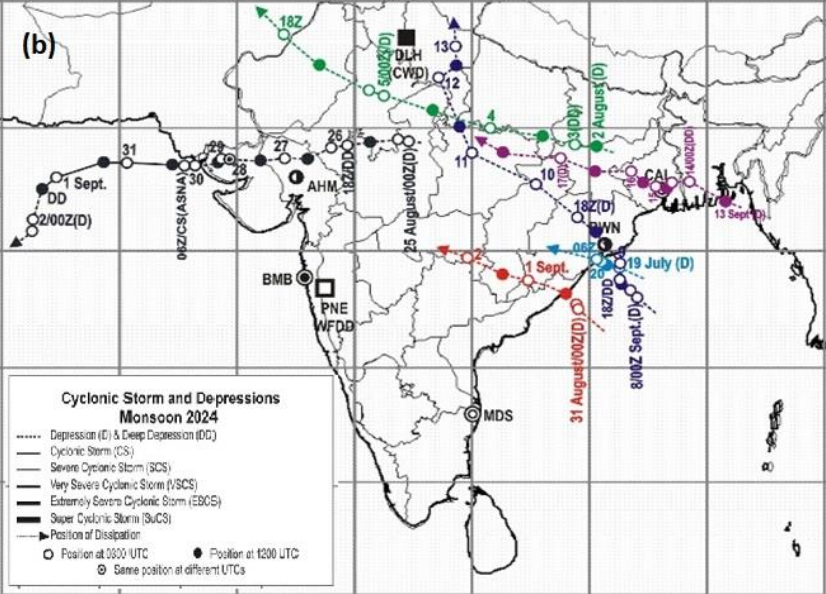
\includegraphics[width=1.35\linewidth]{../images/IMD-report-2024.png}
		\end{figure}
		{\tiny \textbf{Fig.\ 2:} IMD Annual Monsoon Report 2024.}
	\end{columns}
\end{frame}

% -------------------------------------------------------------------
% TODO: Check
\setLayout{plain}
\begin{frame}{Validation - ERA5 detected MD track from IMD Annual Monsoon Report 2024}
	\vspace{-0.2cm}
	\begin{block}{\small Track Details}
		\footnotesize
		\begin{tabular}{p{0.1\linewidth}p{0.2\linewidth}p{0.3\linewidth}p{0.2\linewidth}}
			\toprule
			\rowcolor{MyBlue!15}
			\textbf{Track} & \textbf{Period} & \textbf{Origin} & \textbf{Duration} ($\geq$96h/Long) \\
			\midrule
			1              & 18–21 Jul       & Ocean-Origin    & 78h / Short                        \\
			2              & 01–06 Aug       & Land-Origin     & 106h / Long                        \\
			3              & 23–29 Aug       & Land-Origin     & 146h / Long                        \\
			4              & 30 Aug–02 Sep   & Ocean-Origin    & 75h / Short                        \\
			5              & 06–13 Sep       & Ocean-Origin    & 165h / Long                        \\
			6              & 13–18 Sep       & Land-Origin     & 117h / Long                        \\
			\bottomrule
		\end{tabular}
	\end{block}

	\vspace{0.2cm}
	\begin{alertblock}{\small Validation Result}
		\footnotesize
		Minor $\pm$6–12h differences in start/end times arise from
		ERA5 hourly vs.\ IMD 3-hourly resolution.
		Mean detected duration: $\mathbf{115.2 \pm 38.3}$ hours.
	\end{alertblock}
\end{frame}

% -------------------------------------------------------------------
% --- TRACK 1 -------------------------------------------------
\subsection{Track 1 Short-lived, Ocean-Origin, July}
\setLayout{plain}
\begin{frame}{Track 1 - Short-lived, Ocean-Origin, July}
	\vspace{-0.5cm}
	\begin{center}
		\begin{columns}[T]
			\column{0.5\textwidth}
			\includegraphics[width=0.9\textwidth]{../../../version26-with-ocean-masking-lsm/output_2024/track_1/MD_track_1_detailed.png}

			\begin{block}{\small Statistics}
				\begin{itemize}\footnotesize
					\item \textbf{Period:} 18 Jul 04:00 – 21 Jul 07:00, 2024
					\item \textbf{Duration} : 78 hours ($\sim$ 3 days)
					\item \textbf{Category} : short-lived MD
					\item \textbf{Origin} : Bay of Bengal (Oceanic)
					\item \textbf{Path:} Ocean $\to$ Eastern Ghats / Odisha coast
				\end{itemize}
			\end{block}

			\column{0.5\textwidth}
			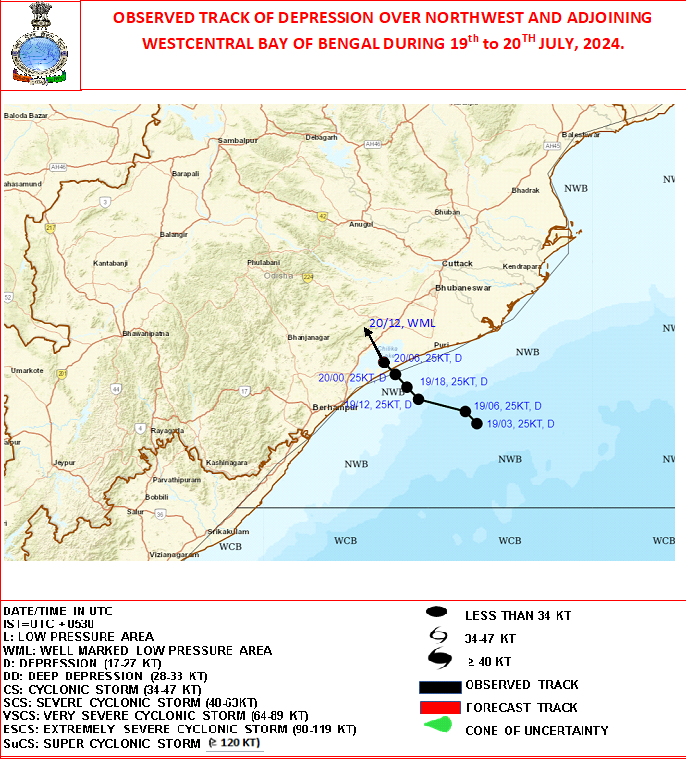
\includegraphics[width=0.8\textwidth]{../images/July-19-20-2024.png}

			{\tiny RSMC New Delhi Report 2024}\footnote{\tiny Source RSMC New Delhi Report 2024 : \href{https://rsmcnewdelhi.imd.gov.in/report.php?internal\_menu=MzQ=}{\url{https://rsmcnewdelhi.imd.gov.in/report.php?internal\_menu=MzQ=}}}
		\end{columns}
	\end{center}
\end{frame}

% -------------------------------------------------------------------
\subsubsection{Track 1 Translation Speed}
\setLayout{horizontal}
\begin{frame}{Track 1 - Translation Speed of MD Center}
	\begin{center}
		\includegraphics[width=0.8\textwidth]{../../../version26-with-ocean-masking-lsm/output_2024/track_1/translational-speed/track_1_speed_ms.png}
	\end{center}
\end{frame}

% -------------------------------------------------------------------
\setLayout{plain}
\begin{frame}{Track 1 - Heat Flux \&  Precipitation \& Soil Moisture Time Evolution}
	\begin{columns}[T]
		\column{0.50\textwidth}
		\vspace{-0.3cm}
		\begin{figure}
			\centering
			\includegraphics[width=1.1\textwidth]{../../../version26-with-ocean-masking-lsm/output_2024/track_1/time_series/track_1_heat_flux_time_series.png}
		\end{figure}
		{\tiny \textbf{Fig.\ 3:} SHF, LHF, THF time series for Track 1.
		Landfall transition: LHF decreases markedly as the system loses oceanic moisture supply.}

		\column{0.50\textwidth}
		\vspace{-0.3cm}
		\begin{figure}
			\centering
			\includegraphics[width=1.1\textwidth]{../../version25-with-ocean-masking-lsm/output_2024/track_1/time_series/track_1_TP-SWVL1_time_series.png}
		\end{figure}
		{\tiny \textbf{Fig.\ 4:} TP and SWVL1 evolution.
		TP pulse after landfall translate to sustained SWVL1 increase.}
	\end{columns}
\end{frame}

% -------------------------------------------------------------------
\setLayout{plain}
\begin{frame}{Track 1 - Heat Flux \&  Precipitation \& Soil Moisture Time Evolution}
	\begin{columns}[T]
		\column{0.50\textwidth}
		\vspace{-0.3cm}
		\begin{figure}
			\centering
			\includegraphics[width=1.1\textwidth]{../../../version26-with-ocean-masking-lsm/output_2024/track_1/time_series/track_1_heat_flux_time_series.png}
		\end{figure}
		{\tiny \textbf{Fig:} Heat flux evolution, Track 1. Clear diurnal SHF oscillations throughout land phase confirm active boundary layer coupling and not due to ocean-phase suppression.}

		\column{0.50\textwidth}
		\vspace{-0.3cm}
		\begin{figure}
			\centering
			\includegraphics[width=1.1\textwidth]{../../version25-with-ocean-masking-lsm/output_2024/track_1/time_series/track_1_TP-SWVL1_time_series.png}
		\end{figure}
		{\tiny \textbf{Fig.:} TP and SWVL1 for Track 1.
		High baseline SWVL1 ($\sim$0.4 m$^3$/m$^3$) supports sustained feedback even as individual TP pulses fluctuate.}
	\end{columns}
\end{frame}

% -------------------------------------------------------------------
\subsubsection{Track 1 Relation}
\setLayout{plain}
\begin{frame}{Track 1 Soil Moisture heat flux relation(\texttt{SWVL1-HF}), Precipitation Soil moisture relation (\texttt{TP-SWVL1}) and Precipitation Heat Flux (\texttt{TP-HF}) Relation}
	\vspace{-0.3cm}
	\begin{columns}[t]
		\begin{column}{0.5\textwidth}
			\begin{center}
				\includegraphics[width=1.1\textwidth]{../../version26-with-ocean-masking-lsm/output_2024/track_1/correlation_analysis/relation/track_1_SWVL1-HF_relation.png} \\
				\includegraphics[width=1.1\textwidth]{../../version26-with-ocean-masking-lsm/output_2024/track_1/correlation_analysis/relation/track_1_TP-HF_relation.png}
			\end{center}
		\end{column}

		\begin{column}{0.5\textwidth}
			\begin{center}
				\includegraphics[width=1.1\textwidth]{../../version26-with-ocean-masking-lsm/output_2024/track_1/correlation_analysis/relation/track_1_TP-SWVL1_relation.png}
			\end{center}
		\end{column}
	\end{columns}
\end{frame}

% -------------------------------------------------------------------
\setLayout{plain}
\begin{frame}{Track 1 Soil Moisture Heat Flux (\texttt{SWVL1-HF}) and Precipitation Soil moisture (\texttt{TP-SWVL1}) Lag Relation}
	\vspace{-0.3cm}
	\begin{columns}[t]
		\begin{column}{0.5\textwidth}
			\begin{center}
				\includegraphics[width=\textwidth]{../../version26-with-ocean-masking-lsm/output_2024/track_1/correlation_analysis/lag_relation/track_1_SWVL1-LHF_lag_relation.png} \\
				\includegraphics[width=\textwidth]{../../version26-with-ocean-masking-lsm/output_2024/track_1/correlation_analysis/lag_relation/track_1_SWVL1-SHF_lag_relation.png}
			\end{center}
		\end{column}

		\begin{column}{0.5\textwidth}
			\begin{center}
				\includegraphics[width=\textwidth]{../../version26-with-ocean-masking-lsm/output_2024/track_1/correlation_analysis/lag_relation/track_1_TP-SWVL1_lag_relation.png}
			\end{center}
		\end{column}
	\end{columns}
\end{frame}

\setLayout{plain}
\begin{frame}{Track 1 Lag relations}
	\vspace{-0.3cm}
	\begin{columns}[t]
		\begin{column}{0.5\textwidth}
			\begin{center}
				\includegraphics[width=\textwidth]{../../version26-with-ocean-masking-lsm/output_2024/track_1/correlation_analysis/lag_relation/track_1_TP-LHF_lag_relation.png} \\
				\includegraphics[width=\textwidth]{../../version26-with-ocean-masking-lsm/output_2024/track_1/correlation_analysis/lag_relation/track_1_TP-SHF_lag_relation.png}
			\end{center}
		\end{column}
	\end{columns}
\end{frame}

% % -------------------------------------------------------------------
% \setLayout{plain}
% \begin{frame}{Track 1 - TP–SWVL1 Relation \& Lag Correlation}
% 	\begin{columns}[T]
% 		\column{0.50\textwidth}
% 		\vspace{-0.3cm}
% 		\begin{figure}
% 			\centering
% 			\includegraphics[width=\textwidth]{../../version26-with-ocean-masking-lsm/output_2024/track_1/correlation_analysis/relation/track_1_TP-SWVL1_relation.png}
% 		\end{figure}
% 		{\tiny \textbf{Fig.\ 5:} TP–SWVL1 scatter. Weak negative relation
% 		($r \approx -0.26$, $p < 0.05$) - rainfall leads to temporary
% 		saturation then rapid drainage; no sustained feedback.}
%
% 		\column{0.50\textwidth}
% 		\vspace{-0.3cm}
% 		\begin{figure}
% 			\centering
% 			\includegraphics[width=\textwidth]{../../version26-with-ocean-masking-lsm/output_2024/track_1/correlation_analysis/lag_relation/track_1_TP-SWVL1_lag_relation.png}
% 		\end{figure}
% 		{\tiny \textbf{Fig.\ 6:} Lag correlation TP vs.\ SWVL1.
% 		Peak at +24h lag indicates a \textit{diurnal antecedent moisture cycle}
% 		rather than a positive feedback - soil moisture leads rain by one day
% 		but the loop is not self-sustaining.}
% 	\end{columns}
% \end{frame}
%
% % -------------------------------------------------------------------
% \setLayout{plain}
% \begin{frame}{Track 1 - Translation Speed \& Elevation}
% 	\begin{columns}[T]
% 		\column{0.50\textwidth}
% 		\vspace{-0.3cm}
% 		\begin{figure}
% 			\centering
% 			\includegraphics[width=0.95\textwidth]{../../version26-with-ocean-masking-lsm/output_2024/track_1/translational-speed/track_1_speed_ms.png}
% 		\end{figure}
% 		{\tiny \textbf{Fig.\ 7:} Translation speed (m/s) for Track 1.
% 		Speed spikes correspond to interaction with monsoon steering flow.
% 		Rapid movement limits time for soil moisture recharge.}
%
% 		\column{0.50\textwidth}
% 		\vspace{-0.3cm}
% 		\begin{figure}
% 			\centering
% 			\includegraphics[width=0.95\textwidth]{../../version26-with-ocean-masking-lsm/output_2024/track_1/elevation_analysis/MD_track_1_elevation_mosaic.png}
% 		\end{figure}
% 		{\tiny \textbf{Fig.\ 8:} SRTM elevation mosaic along Track 1.
% 		Track traverses Eastern Ghats - elevated terrain (600–1400 m)
% 		accelerates drainage and breaks the TP–SWVL1 feedback.}
% 	\end{columns}
% \end{frame}

% -------------------------------------------------------------------
\subsubsection{Track 1 Hovm\"oller}
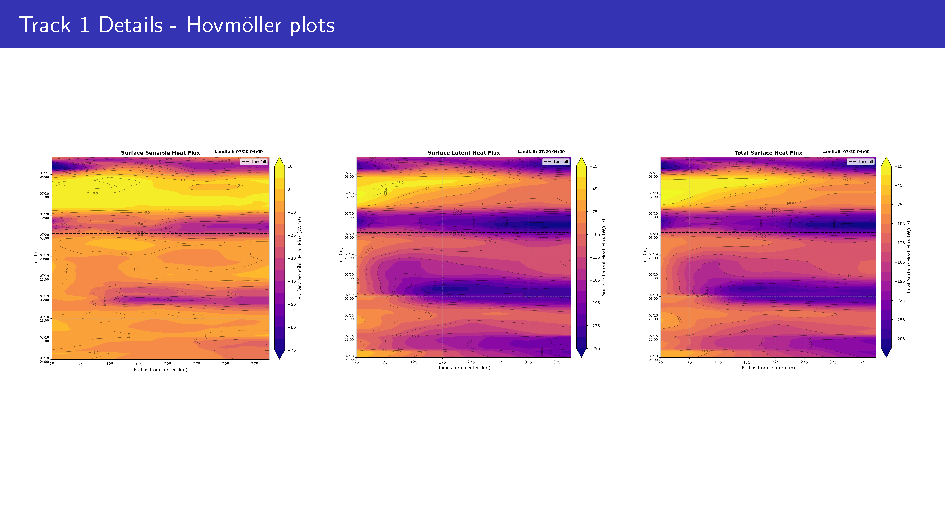
\includepdf[
	pages=-,
	scale=1,
	frame=true,
	pagecommand={\stepcounter{framenumber}},
	offset=0mm 0mm
]{../slides/hov-1.pdf}

% -------------------------------------------------------------------
\subsubsection{Track 1 SRTM Elevation Map}
\setLayout{plain}
\begin{frame}{Track 1 SRTM Elevation Map}
	\vspace{-0.3cm}
	\begin{center}
		\includegraphics[width=0.6\textwidth]{../../version26-with-ocean-masking-lsm/output_2024/track_1/elevation_analysis/MD_track_1_elevation_mosaic.png}
	\end{center}
\end{frame}
%
% --- TRACK 2 -------------------------------------------------
\subsection{Track 2 Long-lived, Land-Origin, August}
\setLayout{plain}
\begin{frame}{Track 2 - Long-lived, Land-Origin, August}
	\vspace{-0.5cm}
	\begin{center}
		\begin{columns}[T]
			\column{0.5\textwidth}
			\includegraphics[width=0.9\textwidth]{../../../version26-with-ocean-masking-lsm/output_2024/track_2/MD_track_2_detailed.png}

			\begin{block}{\small Statistics}
				\begin{itemize}\footnotesize
					\item \textbf{Period:} 01 Aug 19:00 – 06 Aug 04:00, 2024
					\item \textbf{Duration:} 106 h ($\sim$4.5 days)
					\item \textbf{Category} : Long-lived MD
					\item \textbf{Origin:} Over land (Madhya Pradesh / Deep Depression)
				\end{itemize}
			\end{block}

			\column{0.5\textwidth}
			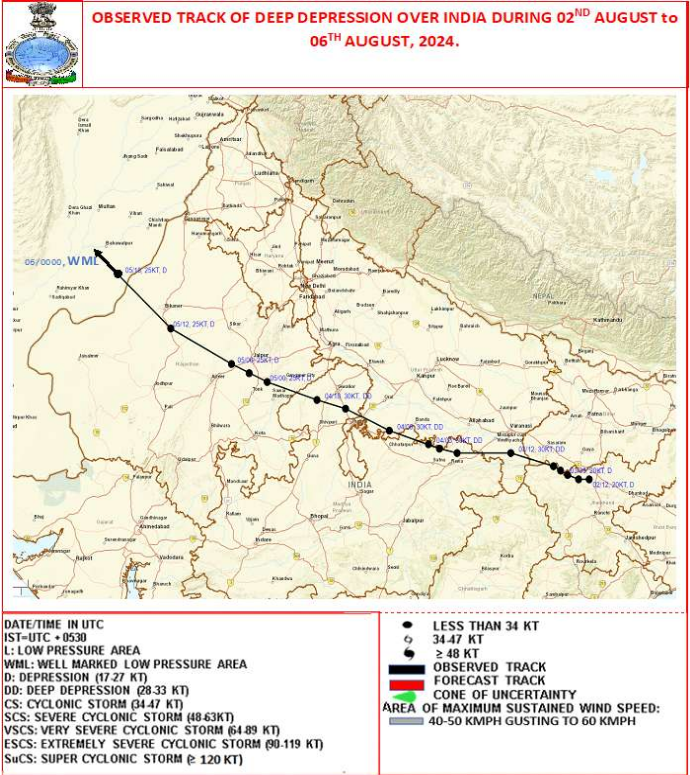
\includegraphics[width=0.8\textwidth]{../images/August-02-06-2024.png}

			{\tiny RSMC New Delhi Report 2024}% \footnote{\tiny Source RSMC New Delhi Report 2024 : \href{https://rsmcnewdelhi.imd.gov.in/report.php?internal\_menu=MzQ=}{\url{https://rsmcnewdelhi.imd.gov.in/report.php?internal\_menu=MzQ=}}}
		\end{columns}

		\begin{block}{\footnotesize Physical Interpretation}
			\scriptsize Land-origin Deep Depression. Madhya Pradesh clay soils retain
			moisture efficiently $\to$ sustained LHF $\to$ long inland survival.
			The ``Deep Depression'' status far from coast is direct evidence
			of land-surface flux acting as secondary energy source.
		\end{block}
	\end{center}
\end{frame}

% -------------------------------------------------------------------
\subsubsection{Track 2 Translation Speed}
\begin{frame}{Track 2 - Translation Speed of MD Center}
	\begin{center}
		\includegraphics[width=0.8\textwidth]{../../../version26-with-ocean-masking-lsm/output_2024/track_2/translational-speed/track_2_speed_ms.png}
	\end{center}
\end{frame}

% -------------------------------------------------------------------
\setLayout{plain}
\begin{frame}{Track 2 - Heat Flux \&  Precipitation \& Soil Moisture Time Evolution}
	\begin{columns}[T]
		\column{0.50\textwidth}
		\vspace{-0.3cm}
		\begin{figure}
			\centering
			\includegraphics[width=1.1\textwidth]{../../../version26-with-ocean-masking-lsm/output_2024/track_2/time_series/track_2_heat_flux_time_series.png}
		\end{figure}
		{\tiny \textbf{Fig.\ 9:} Heat flux time series for Track 2.
		Land-origin track shows sustained positive SHF (diurnal pumping)
		throughout - no ocean-phase suppression.}

		\column{0.50\textwidth}
		\vspace{-0.3cm}
		\begin{figure}
			\centering
			\includegraphics[width=1.1\textwidth]{../../version25-with-ocean-masking-lsm/output_2024/track_2/time_series/track_2_TP-SWVL1_time_series.png}
		\end{figure}
		{\tiny \textbf{Fig.\ 10:} TP and SWVL1 for Track 2.
		High baseline SWVL1 ($\sim$0.45 m$^3$/m$^3$) supports sustained feedback even as individual TP pulses fluctuate.}
	\end{columns}
\end{frame}

% -------------------------------------------------------------------
\subsubsection{Track 2 Relation}
\setLayout{plain}
\begin{frame}{Track 2 Soil Moisture heat flux relation(\texttt{SWVL1-HF}), Precipitation Soil moisture relation (\texttt{TP-SWVL1}) and Precipitation Heat Flux (\texttt{TP-HF}) Relation}
	\vspace{-0.3cm}
	\begin{columns}[t]
		\begin{column}{0.5\textwidth}
			\begin{center}
				\includegraphics[width=1.1\textwidth]{../../version26-with-ocean-masking-lsm/output_2024/track_2/correlation_analysis/relation/track_2_SWVL1-HF_relation.png} \\
				\includegraphics[width=1.1\textwidth]{../../version26-with-ocean-masking-lsm/output_2024/track_2/correlation_analysis/relation/track_2_TP-HF_relation.png}
			\end{center}
		\end{column}

		\begin{column}{0.5\textwidth}
			\begin{center}
				\includegraphics[width=1.1\textwidth]{../../version26-with-ocean-masking-lsm/output_2024/track_2/correlation_analysis/relation/track_2_TP-SWVL1_relation.png}
			\end{center}
		\end{column}
	\end{columns}
\end{frame}

% -------------------------------------------------------------------
\setLayout{plain}
\begin{frame}{Track 2 Soil Moisture Heat Flux (\texttt{SWVL1-HF}) and Precipitation Soil moisture (\texttt{TP-SWVL1}) Lag Relation}
	\vspace{-0.3cm}
	\begin{columns}[t]
		\begin{column}{0.5\textwidth}
			\begin{center}
				\includegraphics[width=\textwidth]{../../version26-with-ocean-masking-lsm/output_2024/track_2/correlation_analysis/lag_relation/track_2_SWVL1-LHF_lag_relation.png} \\
				\includegraphics[width=\textwidth]{../../version26-with-ocean-masking-lsm/output_2024/track_2/correlation_analysis/lag_relation/track_2_SWVL1-SHF_lag_relation.png}
			\end{center}
		\end{column}

		\begin{column}{0.5\textwidth}
			\begin{center}
				\includegraphics[width=\textwidth]{../../version26-with-ocean-masking-lsm/output_2024/track_2/correlation_analysis/lag_relation/track_2_TP-SWVL1_lag_relation.png}
			\end{center}
		\end{column}
	\end{columns}
\end{frame}

\setLayout{plain}
\begin{frame}{Track 2 Lag relations}
	\vspace{-0.3cm}
	\begin{columns}[t]
		\begin{column}{0.5\textwidth}
			\begin{center}
				\includegraphics[width=\textwidth]{../../version26-with-ocean-masking-lsm/output_2024/track_2/correlation_analysis/lag_relation/track_2_TP-LHF_lag_relation.png} \\
				\includegraphics[width=\textwidth]{../../version26-with-ocean-masking-lsm/output_2024/track_2/correlation_analysis/lag_relation/track_2_TP-SHF_lag_relation.png}
			\end{center}
		\end{column}
	\end{columns}
\end{frame}

% -------------------------------------------------------------------
\subsubsection{Track 2 Hovm\"oller}
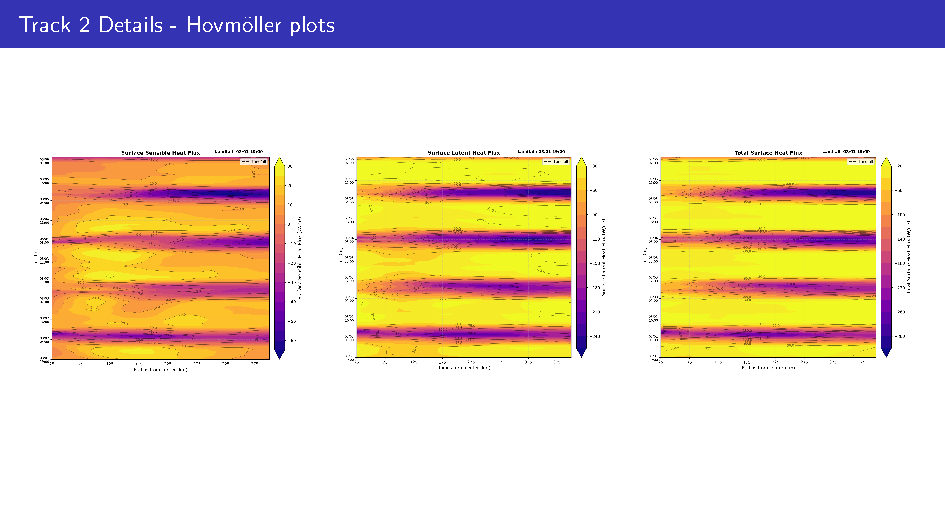
\includepdf[
	pages=-,
	scale=1,
	frame=true,
	pagecommand={\stepcounter{framenumber}},
	offset=0mm 0mm
]{../slides/hov-2.pdf}

% -------------------------------------------------------------------
\subsubsection{Track 2 SRTM Elevation Map}
\setLayout{plain}
\begin{frame}{Track 2 SRTM Elevation Map}
	\vspace{-0.3cm}
	\begin{center}
		\includegraphics[width=0.6\textwidth]{../../version26-with-ocean-masking-lsm/output_2024/track_2/elevation_analysis/MD_track_2_elevation_mosaic.png}
	\end{center}
\end{frame}

% --- TRACK 3 -------------------------------------------------
\subsection{Track 3 Long-lived, Land-Origin, August}
\setLayout{plain}
\begin{frame}{Track 3 - Long-lived, Land-Origin, August}
	\vspace{-0.5cm}
	\begin{center}
		\begin{columns}[T]
			\column{0.5\textwidth}
			\includegraphics[width=0.9\textwidth]{../../../version26-with-ocean-masking-lsm/output_2024/track_3/MD_track_3_detailed.png}

			\begin{block}{\small Statistics}
				\begin{itemize}\footnotesize
					\item \textbf{Period:} 23 Aug 08:00 – 29 Aug 10:00, 2024
					\item \textbf{Duration:} 146 h ($\sim$6 days)
					\item \textbf{Category} : Long-lived MD
					\item \textbf{Origin:} Over land (Central India / Deep Depression)
				\end{itemize}
			\end{block}

			\column{0.5\textwidth}
			% no RSMC image
		\end{columns}

		% \vspace{0.2cm}
		% \begin{alertblock}{\small Key Finding}
		% 	\scriptsize
		% 	Best combination of high moisture capacity + moderate memory + strongest
		% 	coupling $\to$ highest CE among all tracks. Validates H1 and H3: wet soil
		%       $\to$ strong FSI $\to$ long survival. 
		% \end{alertblock}
	\end{center}
\end{frame}

% -------------------------------------------------------------------
\subsubsection{Track 3 Translation Speed}
\begin{frame}{Track 3 - Translation Speed of MD Center}
	\begin{center}
		\includegraphics[width=0.8\textwidth]{../../../version26-with-ocean-masking-lsm/output_2024/track_3/translational-speed/track_3_speed_ms.png}
	\end{center}
\end{frame}

% -------------------------------------------------------------------
\setLayout{plain}
\begin{frame}{Track 3 - Heat Flux \&  Precipitation \& Soil Moisture Time Evolution}
	\begin{columns}[T]
		\column{0.50\textwidth}
		\vspace{-0.3cm}
		\begin{figure}
			\centering
			\includegraphics[width=1.1\textwidth]{../../../version26-with-ocean-masking-lsm/output_2024/track_3/time_series/track_3_heat_flux_time_series.png}
		\end{figure}
		{\tiny \textbf{Fig:} Heat flux evolution, Track 3. Clear diurnal SHF oscillations throughout land phase confirm active boundary layer coupling and not due to ocean-phase suppression.}

		\column{0.50\textwidth}
		\vspace{-0.3cm}
		\begin{figure}
			\centering
			\includegraphics[width=1.1\textwidth]{../../version25-with-ocean-masking-lsm/output_2024/track_3/time_series/track_3_TP-SWVL1_time_series.png}
		\end{figure}
		{\tiny \textbf{Fig.:} TP and SWVL1 for Track 3.
		High baseline SWVL1 ($\sim$0.4 m$^3$/m$^3$) supports sustained feedback even as individual TP pulses fluctuate.}
	\end{columns}
\end{frame}

% -------------------------------------------------------------------
\subsubsection{Track 3 Relation}
\setLayout{plain}
\begin{frame}{Track 6 Soil Moisture heat flux relation(\texttt{SWVL1-HF}), Precipitation Soil moisture relation (\texttt{TP-SWVL1}) and Precipitation Heat Flux (\texttt{TP-HF}) Relation}
	\vspace{-0.3cm}
	\begin{columns}[t]
		\begin{column}{0.5\textwidth}
			\begin{center}
				\includegraphics[width=1.1\textwidth]{../../version26-with-ocean-masking-lsm/output_2024/track_3/correlation_analysis/relation/track_3_SWVL1-HF_relation.png} \\
				\includegraphics[width=1.1\textwidth]{../../version26-with-ocean-masking-lsm/output_2024/track_3/correlation_analysis/relation/track_3_TP-HF_relation.png}
			\end{center}
		\end{column}

		\begin{column}{0.5\textwidth}
			\begin{center}
				\includegraphics[width=1.1\textwidth]{../../version26-with-ocean-masking-lsm/output_2024/track_3/correlation_analysis/relation/track_3_TP-SWVL1_relation.png}
			\end{center}
		\end{column}
	\end{columns}
\end{frame}

% -------------------------------------------------------------------
\setLayout{plain}
\begin{frame}{Track 3 Soil Moisture Heat Flux (\texttt{SWVL1-HF}) and Precipitation Soil moisture (\texttt{TP-SWVL1}) Lag Relation}
	\vspace{-0.3cm}
	\begin{columns}[t]
		\begin{column}{0.5\textwidth}
			\begin{center}
				\includegraphics[width=\textwidth]{../../version26-with-ocean-masking-lsm/output_2024/track_3/correlation_analysis/lag_relation/track_3_SWVL1-LHF_lag_relation.png} \\
				\includegraphics[width=\textwidth]{../../version26-with-ocean-masking-lsm/output_2024/track_3/correlation_analysis/lag_relation/track_3_SWVL1-SHF_lag_relation.png}
			\end{center}
		\end{column}

		\begin{column}{0.5\textwidth}
			\begin{center}
				\includegraphics[width=\textwidth]{../../version26-with-ocean-masking-lsm/output_2024/track_3/correlation_analysis/lag_relation/track_3_TP-SWVL1_lag_relation.png}
			\end{center}
		\end{column}
	\end{columns}
\end{frame}

\setLayout{plain}
\begin{frame}{Track 3 Lag relations}
	\vspace{-0.3cm}
	\begin{columns}[t]
		\begin{column}{0.5\textwidth}
			\begin{center}
				\includegraphics[width=\textwidth]{../../version26-with-ocean-masking-lsm/output_2024/track_3/correlation_analysis/lag_relation/track_3_TP-LHF_lag_relation.png} \\
				\includegraphics[width=\textwidth]{../../version26-with-ocean-masking-lsm/output_2024/track_3/correlation_analysis/lag_relation/track_3_TP-SHF_lag_relation.png}
			\end{center}
		\end{column}
	\end{columns}
\end{frame}

% -------------------------------------------------------------------
\subsubsection{Track 3 Hovm\"oller}
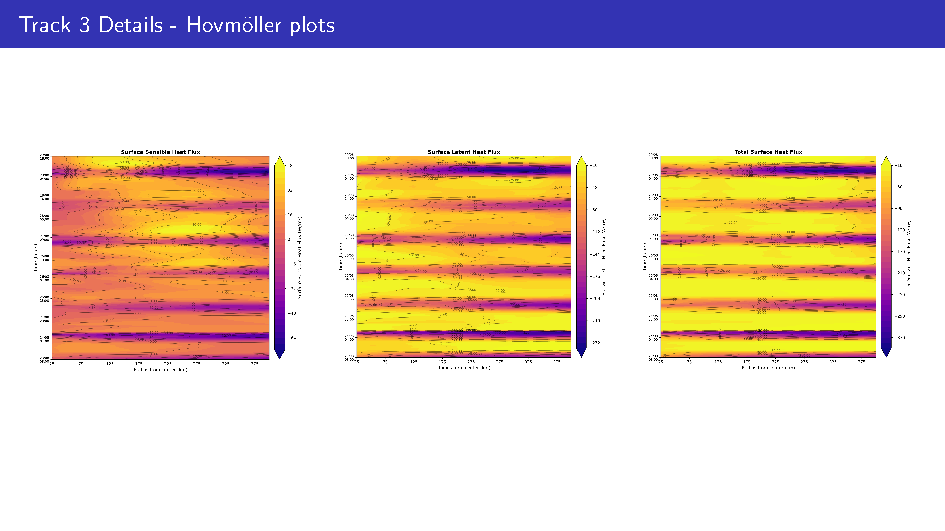
\includepdf[
	pages=-,
	scale=1,
	frame=true,
	pagecommand={\stepcounter{framenumber}},
	offset=0mm 0mm
]{../slides/hov-3.pdf}

% -------------------------------------------------------------------
\subsubsection{Track 3 SRTM Elevation Map}
\setLayout{plain}
\begin{frame}{Track 3 SRTM Elevation Map}
	\vspace{-0.3cm}
	\begin{center}
		\includegraphics[width=0.6\textwidth]{../../version26-with-ocean-masking-lsm/output_2024/track_3/elevation_analysis/MD_track_3_elevation_mosaic.png}
	\end{center}
\end{frame}

% --- TRACK 4 -------------------------------------------------
\subsection{Track 4 Short-lived, Ocean-Origin / Pre-Cyclone ASNA, August-September}
\setLayout{plain}
\begin{frame}{Track 4 - Short-lived, Ocean-Origin, Pre-Cyclone ASNA, Aug–Sep}
	\vspace{-0.5cm}
	\begin{center}
		\begin{columns}[T]
			\column{0.5\textwidth}
			\includegraphics[width=0.9\textwidth]{../../version26-with-ocean-masking-lsm/output_2024/track_4/MD_track_4_detailed.png}

			\begin{block}{\small Statistics}
				\begin{itemize}\footnotesize
					\item \textbf{Period:} 30 Aug 05:00 – 02 Sep 08:00, 2024
					\item \textbf{Duration:} 75 h ($\sim$3 days)
					\item \textbf{Category} : Short--lived MD
					\item \textbf{Origin:} Bay of Bengal (Oceanic)
					\item \textbf{Path:} Ocean $\to$ Eastern Ghats
				\end{itemize}
			\end{block}

			\column{0.5\textwidth}
			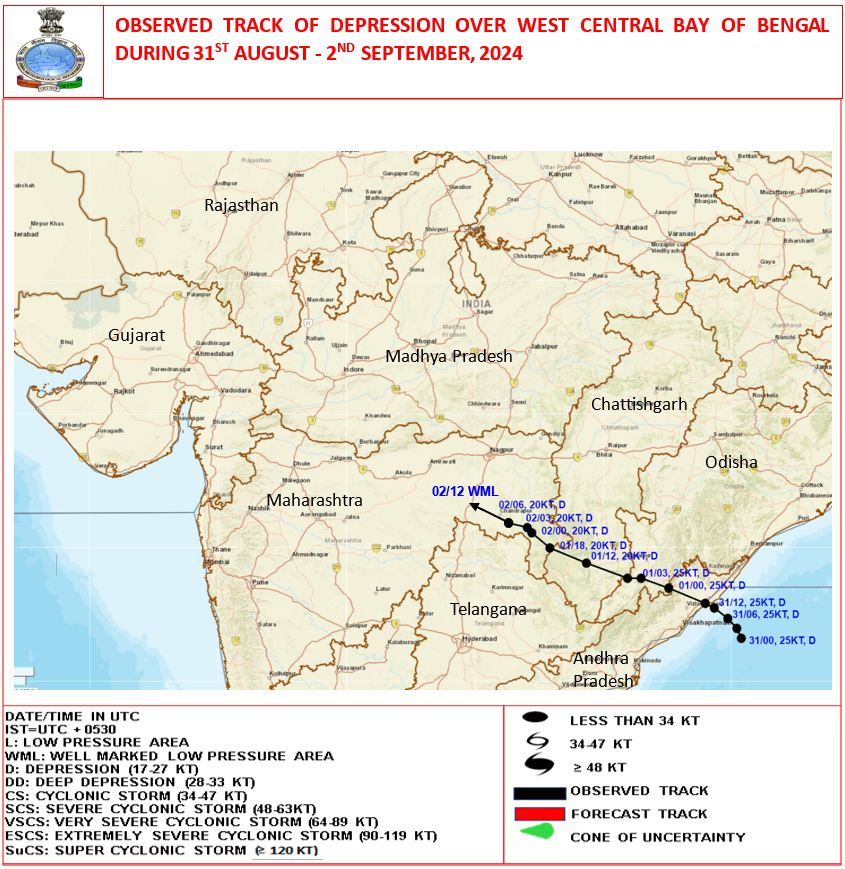
\includegraphics[width=0.8\textwidth]{../images/August-31-Sep-02-2024.png}

			{\tiny RSMC New Delhi Report 2024}% \footnote{\tiny Source RSMC New Delhi Report 2024 : \href{https://rsmcnewdelhi.imd.gov.in/report.php?internal\_menu=MzQ=}{\url{https://rsmcnewdelhi.imd.gov.in/report.php?internal\_menu=MzQ=}}}
		\end{columns}

		\begin{alertblock}{\footnotesize The Control Case}
			\scriptsize Despite higher intensity (Cyclone status), longevity was limited by absence
			of inland soil moisture feedback. Rapid coastal runoff (sandy soils) and high elevation prevents feedback loop.
		\end{alertblock}
	\end{center}
\end{frame}

% -------------------------------------------------------------------
\subsubsection{Track 4 Translation Speed}
\begin{frame}{Track 4 - Translation Speed of MD Center}
	\begin{center}
		\includegraphics[width=0.8\textwidth]{../../../version26-with-ocean-masking-lsm/output_2024/track_4/translational-speed/track_4_speed_ms.png}
	\end{center}
\end{frame}

% -------------------------------------------------------------------
\setLayout{plain}
\begin{frame}{Track 4 - Heat Flux \&  Precipitation \& Soil Moisture Time Evolution}
	\begin{columns}[T]
		\column{0.50\textwidth}
		\vspace{-0.3cm}
		\begin{figure}
			\centering
			\includegraphics[width=1.1\textwidth]{../../../version26-with-ocean-masking-lsm/output_2024/track_4/time_series/track_4_heat_flux_time_series.png}
		\end{figure}
		{\tiny \textbf{Fig:} Heat flux evolution, Track 4. Diurnal SHF oscillations over land phase}

		\column{0.50\textwidth}
		\vspace{-0.3cm}
		\begin{figure}
			\centering
			\includegraphics[width=1.1\textwidth]{../../version25-with-ocean-masking-lsm/output_2024/track_4/time_series/track_4_TP-SWVL1_time_series.png}
		\end{figure}
		{\tiny \textbf{Fig.:} TP and SWVL1 for Track 4.
		TP pulse after landfall translate to sustained SWVL1 increase.}
	\end{columns}
\end{frame}

% -------------------------------------------------------------------
\subsubsection{Track 4 Relation}
\setLayout{plain}
\begin{frame}{Track 6 Soil Moisture heat flux relation(\texttt{SWVL1-HF}), Precipitation Soil moisture relation (\texttt{TP-SWVL1}) and Precipitation Heat Flux (\texttt{TP-HF}) Relation}
	\vspace{-0.3cm}
	\begin{columns}[t]
		\begin{column}{0.5\textwidth}
			\begin{center}
				\includegraphics[width=1.1\textwidth]{../../version26-with-ocean-masking-lsm/output_2024/track_4/correlation_analysis/relation/track_4_SWVL1-HF_relation.png} \\
				\includegraphics[width=1.1\textwidth]{../../version26-with-ocean-masking-lsm/output_2024/track_4/correlation_analysis/relation/track_4_TP-HF_relation.png}
			\end{center}
		\end{column}

		\begin{column}{0.5\textwidth}
			\begin{center}
				\includegraphics[width=1.1\textwidth]{../../version26-with-ocean-masking-lsm/output_2024/track_4/correlation_analysis/relation/track_4_TP-SWVL1_relation.png}
			\end{center}
		\end{column}
	\end{columns}
\end{frame}

% -------------------------------------------------------------------
\setLayout{plain}
\begin{frame}{Track 5 Soil Moisture Heat Flux (\texttt{SWVL1-HF}) and Precipitation Soil moisture (\texttt{TP-SWVL1}) Lag Relation}
	\vspace{-0.3cm}
	\begin{columns}[t]
		\begin{column}{0.5\textwidth}
			\begin{center}
				\includegraphics[width=\textwidth]{../../version26-with-ocean-masking-lsm/output_2024/track_5/correlation_analysis/lag_relation/track_5_SWVL1-LHF_lag_relation.png} \\
				\includegraphics[width=\textwidth]{../../version26-with-ocean-masking-lsm/output_2024/track_5/correlation_analysis/lag_relation/track_5_SWVL1-SHF_lag_relation.png}
			\end{center}
		\end{column}

		\begin{column}{0.5\textwidth}
			\begin{center}
				\includegraphics[width=\textwidth]{../../version26-with-ocean-masking-lsm/output_2024/track_5/correlation_analysis/lag_relation/track_5_TP-SWVL1_lag_relation.png}
			\end{center}
		\end{column}
	\end{columns}
\end{frame}

\setLayout{plain}
\begin{frame}{Track 4 Lag relations}
	\vspace{-0.3cm}
	\begin{columns}[t]
		\begin{column}{0.5\textwidth}
			\begin{center}
				\includegraphics[width=\textwidth]{../../version26-with-ocean-masking-lsm/output_2024/track_5/correlation_analysis/lag_relation/track_5_TP-LHF_lag_relation.png} \\
				\includegraphics[width=\textwidth]{../../version26-with-ocean-masking-lsm/output_2024/track_5/correlation_analysis/lag_relation/track_5_TP-SHF_lag_relation.png}
			\end{center}
		\end{column}
	\end{columns}
\end{frame}

% -------------------------------------------------------------------
\subsubsection{Track 4 Hovm\"oller}
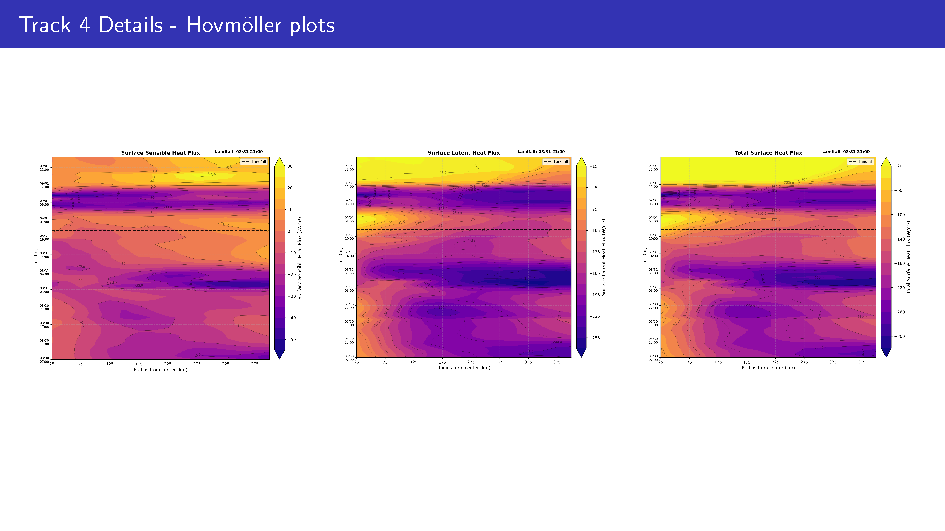
\includepdf[
	pages=-,
	scale=1,
	frame=true,
	pagecommand={\stepcounter{framenumber}},
	offset=0mm 0mm
]{../slides/hov-4.pdf}

% -------------------------------------------------------------------
\subsubsection{Track 4 SRTM Elevation Map}
\setLayout{plain}
\begin{frame}{Track 4 SRTM Elevation Map}
	\vspace{-0.3cm}
	\begin{center}
		\includegraphics[width=0.6\textwidth]{../../version26-with-ocean-masking-lsm/output_2024/track_4/elevation_analysis/MD_track_4_elevation_mosaic.png}
	\end{center}
\end{frame}

% --- TRACK 5 -------------------------------------------------
\subsection{Track 5 Long-lived, Ocean-origin, September}
\setLayout{plain}
\begin{frame}{Track 5 - Long-lived , Ocean-origin, September)}
	\vspace{-0.5cm}
	\begin{center}
		\begin{columns}[T]
			\column{0.5\textwidth}
			\includegraphics[width=0.9\textwidth]{../../version26-with-ocean-masking-lsm/output_2024/track_5/MD_track_5_detailed.png}

			\begin{block}{\small Statistics}
				\begin{itemize}\footnotesize
					\item \textbf{Period:} 06 Sep 06:00 – 13 Sep 03:00, 2024
					\item \textbf{Duration:} 165 h ($\sim$7 days)
					\item \textbf{Category} : Long-lived md
					\item \textbf{Origin:} Bay Of Bengal (oceanic)
				\end{itemize}
			\end{block}

			\column{0.5\textwidth}
			\includegraphics[width=0.8\textwidth]{../images/september-08-10-2024.png}

			{\tiny RSMC New delhi report 2024}% \footnote{\tiny source rsmc new delhi report 2024 : \href{https://rsmcnewdelhi.imd.gov.in/report.php?internal\_menu=mzq=}{\url{https://rsmcnewdelhi.imd.gov.in/report.php?internal\_menu=mzq=}}}
		\end{columns}

		\begin{alertblock}{\footnotesize The anomaly - track 5 survived longest}
			\scriptsize Soil moisture persistence day-to-day sustains the vortex even during weakened coupling.
			Eastern Ghats slowdown (Sep 10) $\to$ vorticity recovers (Sep 11 IMD) $\to$ system re-energises from accumulated soil moisture over plains.
		\end{alertblock}
	\end{center}
\end{frame}

% -------------------------------------------------------------------
\subsubsection{Track 5 Translation Speed}
\begin{frame}{Track 5 - Translation Speed of MD Center}
	\begin{center}
		\includegraphics[width=0.8\textwidth]{../../../version26-with-ocean-masking-lsm/output_2024/track_5/translational-speed/track_5_speed_ms.png}
	\end{center}
\end{frame}

% % -------------------------------------------------------------------
\setLayout{plain}
% 	{\tiny \textbf{Fig.\ 18:} Lag correlation, Track 5.
% 	Near-zero lag ($r = 0.44$) - stable simultaneous feedback loop.
% 	High ACF (0.525) ensures the loop persists between diurnal peaks.}
%
% 	\textbf{Possible explanations for underperforming FSI (observed 0.21 vs.\ predicted 0.40):}
% 	Wind shear suppression during Eastern Ghats encounter $\cdot$
% 	Cooler SST in late-season BoB $\cdot$
% 	Outflow boundary from Track 4 inhibiting convection $\cdot$
% 	Orographic interruption of coupling.
\begin{frame}{Track 5 - Heat Flux, Precipitation \& Soil Moisture Time Evolution}
	\begin{columns}[T]
		\column{0.50\textwidth}
		\vspace{-0.3cm}
		\begin{figure}
			\centering
			\includegraphics[width=1.1\textwidth]{../../../version26-with-ocean-masking-lsm/output_2024/track_5/time_series/track_5_heat_flux_time_series.png}
		\end{figure}
		{\tiny \textbf{Fig:} Heat flux evolution, Track 5. Clear diurnal SHF oscillations throughout land phase confirm active boundary layer coupling and not due to ocean-phase suppression. SHF turns positive over land - the surface actively heats the atmosphere.}

		\column{0.50\textwidth}
		\vspace{-0.3cm}
		\begin{figure}
			\centering
			\includegraphics[width=1.1\textwidth]{../../version25-with-ocean-masking-lsm/output_2024/track_5/time_series/track_5_TP-SWVL1_time_series.png}
		\end{figure}
		{\tiny \textbf{Fig.:} TP and SWVL1 for Track 5.
		TP pulse after landfall translate to sustained SWVL1 increase.}
	\end{columns}
\end{frame}

% -------------------------------------------------------------------
\subsubsection{Track 5 Relation}
\setLayout{plain}
\begin{frame}{Track 5 Soil Moisture heat flux relation(\texttt{SWVL1-HF}), Precipitation Soil moisture relation (\texttt{TP-SWVL1}) and Precipitation Heat Flux (\texttt{TP-HF}) Relation}
	\vspace{-0.3cm}
	\begin{columns}[t]
		\begin{column}{0.5\textwidth}
			\begin{center}
				\includegraphics[width=1.1\textwidth]{../../version26-with-ocean-masking-lsm/output_2024/track_5/correlation_analysis/relation/track_5_SWVL1-HF_relation.png} \\
				\includegraphics[width=1.1\textwidth]{../../version26-with-ocean-masking-lsm/output_2024/track_5/correlation_analysis/relation/track_5_TP-HF_relation.png}
			\end{center}
		\end{column}

		\begin{column}{0.5\textwidth}
			\begin{center}
				\includegraphics[width=1.1\textwidth]{../../version26-with-ocean-masking-lsm/output_2024/track_5/correlation_analysis/relation/track_5_TP-SWVL1_relation.png}
			\end{center}
		\end{column}
	\end{columns}
\end{frame}

% -------------------------------------------------------------------
\setLayout{plain}
\begin{frame}{Track 5 Soil Moisture Heat Flux (\texttt{SWVL1-HF}) and Precipitation Soil moisture (\texttt{TP-SWVL1}) Lag Relation}
	\vspace{-0.3cm}
	\begin{columns}[t]
		\begin{column}{0.5\textwidth}
			\begin{center}
				\includegraphics[width=\textwidth]{../../version26-with-ocean-masking-lsm/output_2024/track_5/correlation_analysis/lag_relation/track_5_SWVL1-LHF_lag_relation.png} \\
				\includegraphics[width=\textwidth]{../../version26-with-ocean-masking-lsm/output_2024/track_5/correlation_analysis/lag_relation/track_5_SWVL1-SHF_lag_relation.png}
			\end{center}
		\end{column}

		\begin{column}{0.5\textwidth}
			\begin{center}
				\includegraphics[width=\textwidth]{../../version26-with-ocean-masking-lsm/output_2024/track_5/correlation_analysis/lag_relation/track_5_TP-SWVL1_lag_relation.png}
			\end{center}
		\end{column}
	\end{columns}
\end{frame}

\setLayout{plain}
\begin{frame}{Track 5 Lag relations}
	\vspace{-0.3cm}
	\begin{columns}[t]
		\begin{column}{0.5\textwidth}
			\begin{center}
				\includegraphics[width=\textwidth]{../../version26-with-ocean-masking-lsm/output_2024/track_5/correlation_analysis/lag_relation/track_5_TP-LHF_lag_relation.png} \\
				\includegraphics[width=\textwidth]{../../version26-with-ocean-masking-lsm/output_2024/track_5/correlation_analysis/lag_relation/track_5_TP-SHF_lag_relation.png}
			\end{center}
		\end{column}
	\end{columns}
\end{frame}

% -------------------------------------------------------------------
\subsubsection{Track 5 Hovm\"oller}
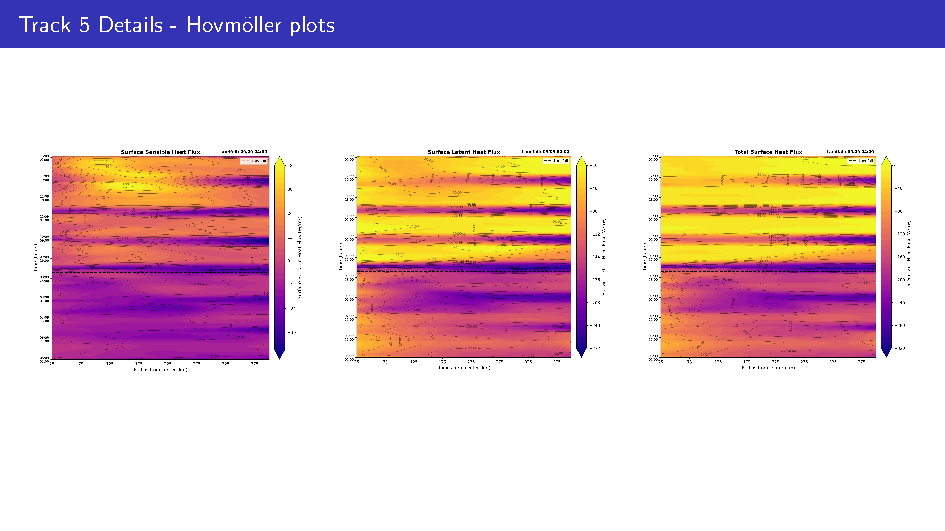
\includepdf[
	pages=-,
	scale=1,
	frame=true,
	pagecommand={\stepcounter{framenumber}},
	offset=0mm 0mm
]{../slides/hov-5.pdf}

% -------------------------------------------------------------------
\subsubsection{Track 5 SRTM Elevation Map}
\setLayout{plain}
\begin{frame}{Track 5 SRTM Elevation Map}
	\vspace{-0.3cm}
	\begin{center}
		\includegraphics[width=0.6\textwidth]{../../version26-with-ocean-masking-lsm/output_2024/track_5/elevation_analysis/MD_track_5_elevation_mosaic.png}
	\end{center}
\end{frame}

% % --- TRACK 6 -------------------------------------------------
\subsection{Track 6 Long-lived, Land-Origin, September}
\setLayout{plain}
\begin{frame}{Track 6 - Long-lived, Land-Origin, September}
	\vspace{-0.5cm}
	\begin{center}
		\begin{columns}[T]
			\column{0.5\textwidth}
			\includegraphics[width=0.9\textwidth]{../../version26-with-ocean-masking-lsm/output_2024/track_6/md_track_6_detailed.png}

			\begin{block}{\small Statistics}
				\begin{itemize}\footnotesize
					\item \textbf{Period:} 13 Sep 12:00 – 18 Sep 07:00, 2024
					\item \textbf{Duration:} 117 h ($\sim$5 days)
					\item \textbf{Origin:} Over land (Eastern India / Deep Depression)
					\item \textbf{Category} : Long-lived md
					\item \textbf{origin:} Bay Of Bengal (oceanic)
				\end{itemize}
			\end{block}

			\column{0.5\textwidth}
			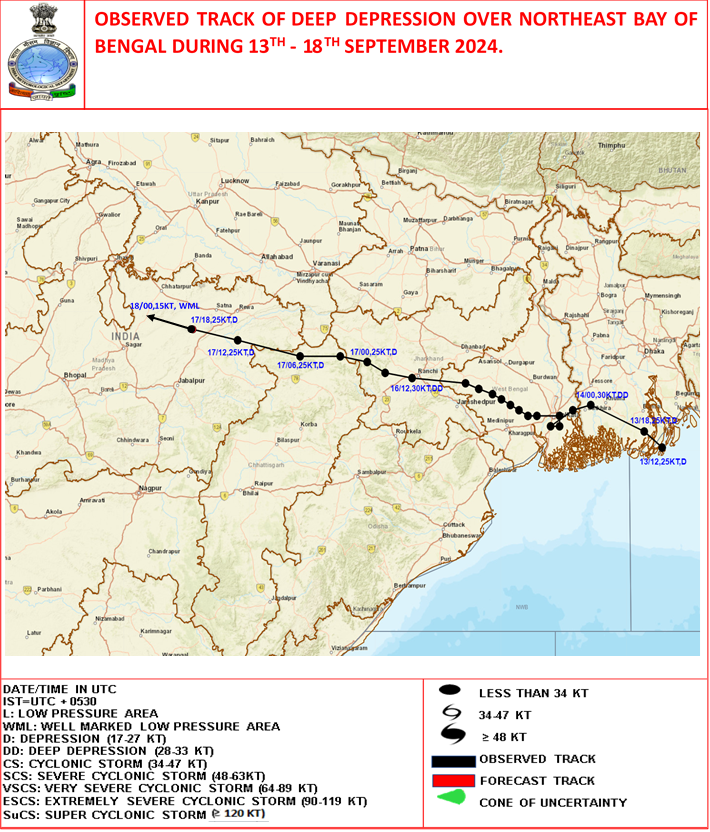
\includegraphics[width=0.8\textwidth]{../images/September-13-18-2024.png}

			{\tiny RSMC New Delhi report 2024}% \footnote{\tiny source rsmc new delhi report 2024 : \href{https://rsmcnewdelhi.imd.gov.in/report.php?internal\_menu=mzq=}{\url{https://rsmcnewdelhi.imd.gov.in/report.php?internal\_menu=mzq=}}}
		\end{columns}

		% \begin{block}{\small Physical Interpretation}
		% 	\scriptsize
		% 	Third consecutive land-origin Deep Depression over Central India.
		% 	Reinforces pattern: Tracks 2, 5, 6 over Madhya Pradesh exhibit
		% 	consistent feedback loops, intensifying into ``Deep'' systems
		% 	far from coast. Saturated soil (ACF near 0) means minimal
		% 	additional memory needed - soil is already at capacity.
		% \end{block}
	\end{center}
\end{frame}

% -------------------------------------------------------------------
\subsubsection{Track 6 Translation Speed}
\begin{frame}{Track 6 Translation Speed of MD Center}
	\begin{center}
		\includegraphics[width=0.8\textwidth]{../../../version26-with-ocean-masking-lsm/output_2024/track_6/translational-speed/track_6_speed_ms.png}
	\end{center}
\end{frame}

% -------------------------------------------------------------------
\setLayout{plain}
\begin{frame}{Track 6 - Heat Flux \&  Precipitation \& Soil Moisture Time Evolution}
	\begin{columns}[T]
		\column{0.50\textwidth}
		\vspace{-0.3cm}
		\begin{figure}
			\centering
			\includegraphics[width=1.1\textwidth]{../../../version26-with-ocean-masking-lsm/output_2024/track_6/time_series/track_6_heat_flux_time_series.png}
		\end{figure}
		{\tiny \textbf{Fig:} Heat flux evolution, Track 6. Clear diurnal SHF oscillations throughout land phase confirm active boundary layer coupling and not due to ocean-phase suppression.}

		\column{0.50\textwidth}
		\vspace{-0.3cm}
		\begin{figure}
			\centering
			\includegraphics[width=1.1\textwidth]{../../version25-with-ocean-masking-lsm/output_2024/track_6/time_series/track_6_TP-SWVL1_time_series.png}
		\end{figure}
		{\tiny \textbf{Fig.:} TP and SWVL1 for Track 6.
		High baseline SWVL1 ($\sim$0.4 m$^3$/m$^3$) supports sustained feedback even as individual TP pulses fluctuate. TP pulse after landfall translate to sustained SWVL1 increase.}
	\end{columns}
\end{frame}

% -------------------------------------------------------------------
\subsubsection{Track 6 Relation}
\setLayout{plain}
\begin{frame}{Track 6 Soil Moisture heat flux relation(\texttt{SWVL1-HF}), Precipitation Soil moisture relation (\texttt{TP-SWVL1}) and Precipitation Heat Flux (\texttt{TP-HF}) Relation}
	\vspace{-0.3cm}
	\begin{columns}[t]
		\begin{column}{0.5\textwidth}
			\begin{center}
				\includegraphics[width=1.1\textwidth]{../../version26-with-ocean-masking-lsm/output_2024/track_6/correlation_analysis/relation/track_6_SWVL1-HF_relation.png} \\
				\includegraphics[width=1.1\textwidth]{../../version26-with-ocean-masking-lsm/output_2024/track_6/correlation_analysis/relation/track_6_TP-HF_relation.png}
			\end{center}
		\end{column}

		\begin{column}{0.5\textwidth}
			\begin{center}
				\includegraphics[width=1.1\textwidth]{../../version26-with-ocean-masking-lsm/output_2024/track_6/correlation_analysis/relation/track_6_TP-SWVL1_relation.png}
			\end{center}
		\end{column}
	\end{columns}
\end{frame}

% -------------------------------------------------------------------
\setLayout{plain}
\begin{frame}{Track 6 Soil Moisture Heat Flux (\texttt{SWVL1-HF}) and Precipitation Soil moisture (\texttt{TP-SWVL1}) Lag Relation}
	\vspace{-0.3cm}
	\begin{columns}[t]
		\begin{column}{0.5\textwidth}
			\begin{center}
				\includegraphics[width=\textwidth]{../../version26-with-ocean-masking-lsm/output_2024/track_6/correlation_analysis/lag_relation/track_6_SWVL1-LHF_lag_relation.png} \\
				\includegraphics[width=\textwidth]{../../version26-with-ocean-masking-lsm/output_2024/track_6/correlation_analysis/lag_relation/track_6_SWVL1-SHF_lag_relation.png}
			\end{center}
		\end{column}

		\begin{column}{0.5\textwidth}
			\begin{center}
				\includegraphics[width=\textwidth]{../../version26-with-ocean-masking-lsm/output_2024/track_6/correlation_analysis/lag_relation/track_6_TP-SWVL1_lag_relation.png}
			\end{center}
		\end{column}
	\end{columns}
\end{frame}

\setLayout{plain}
\begin{frame}{Track 6 Lag relations}
	\vspace{-0.3cm}
	\begin{columns}[t]
		\begin{column}{0.5\textwidth}
			\begin{center}
				\includegraphics[width=\textwidth]{../../version26-with-ocean-masking-lsm/output_2024/track_6/correlation_analysis/lag_relation/track_6_TP-LHF_lag_relation.png} \\
				\includegraphics[width=\textwidth]{../../version26-with-ocean-masking-lsm/output_2024/track_6/correlation_analysis/lag_relation/track_6_TP-SHF_lag_relation.png}
			\end{center}
		\end{column}
	\end{columns}
\end{frame}

% -------------------------------------------------------------------
\subsubsection{Track 6 Hovm\"oller}
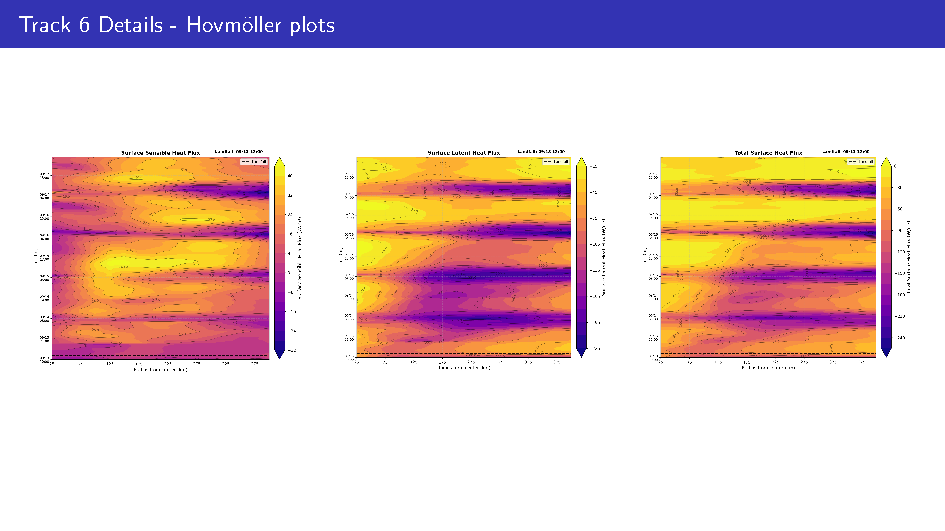
\includepdf[
	pages=-,
	scale=1,
	frame=true,
	pagecommand={\stepcounter{framenumber}},
	offset=0mm 0mm
]{../slides/hov-6.pdf}

% -------------------------------------------------------------------
\subsubsection{Track 6 SRTM Elevation Map}
\setLayout{plain}
\begin{frame}{Track 6 SRTM Elevation Map}
	\vspace{-0.3cm}
	\begin{center}
		\includegraphics[width=0.6\textwidth]{../../version26-with-ocean-masking-lsm/output_2024/track_6/elevation_analysis/MD_track_6_elevation_mosaic.png}
	\end{center}
\end{frame}

% % -------------------------------------------------------------------
% \section{Observations \& Analysis}
% \setLayout{mainpoint}
% \begin{frame}{}
% 	\frametitle{OBSERVATIONS \& ANALYSIS}
% \end{frame}
%
% % -------------------------------------------------------------------
% \subsection{Statistical Summary}
% \setLayout{horizontal}
% \begin{frame}{Cross-Track Statistical Summary - All Coupling Metrics}
% 	\begin{columns}
% 		\column{0.62\textwidth}
% 		\vspace{-0.3cm}
% 		\begin{table}
% 			\centering
% 			\footnotesize
% 			\caption{Coupling metrics for all 6 MD tracks, 2024}
% 			\begin{tabular}{lccccccc}
% 				\toprule
% 				\rowcolor{MyBlue!15}
% 				\textbf{Track} & \textbf{ASM} & \textbf{FSI} & \textbf{ACF} & \textbf{CE} & \textbf{TSI} & \textbf{Dur (h)} & \textbf{Category} \\
% 				\midrule
% 				1              & 0.198        & 0.027        & $-$0.092     & 2.11        & 0.21         & 78               & Weakly coupled    \\
% 				2              & 0.355        & 0.492        & $-$0.061     & 10.37       & 0.44         & 106              & Strongly coupled  \\
% 				3              & 0.389        & 0.604        & $+$0.321     & 15.35       & 0.71         & 146              & Strongly coupled  \\
% 				4              & 0.258        & 0.034        & $-$0.197     & 3.68        & 0.18         & 75               & Weakly coupled    \\
% 				5              & 0.319        & 0.210        & $+$0.525     & 7.61        & 0.39         & 165              & Memory-sustained  \\
% 				6              & 0.378        & 0.402        & $+$0.034     & 10.74       & 0.41         & 117              & Strongly coupled  \\
% 				\midrule
% 				\textbf{Mean}  & 0.316        & 0.295        & 0.088        & 8.31        & 0.39         & 115              &                   \\
% 				\bottomrule
% 			\end{tabular}
% 		\end{table}
%
% 		\column{0.38\textwidth}
% 		\vspace{-0.3cm}
% 		\begin{block}{\small Key Findings}
% 			\footnotesize
% 			\begin{itemize}
% 				\item \textbf{FSI threshold:} Tracks with FSI $>$ 0.4 (T2, T3, T6)
% 				      survive $\geq$105 h. FSI $<$ 0.1 (T1, T4) $\to$ 70–78 h.
% 				\item \textbf{Two survival modes:}
% 				      \textit{Efficiency} (CE, Tracks 2/3/6) vs.\
% 				      \textit{Memory} (ACF, Track 5).
% 				\item \textbf{2024 was wet:} 4 of 6 tracks (67\%) in the
% 				      ``wet'' ASM category ($>$0.32 m$^3$/m$^3$).
% 				\item \textbf{Mean TSI = 0.39:} Terrain explains $\sim$39\%
% 				      of variance; SST/shear/humidity explain the rest.
% 			\end{itemize}
% 		\end{block}
% 		\vspace{0.2cm}
% 		\begin{alertblock}{\small Mean Diurnal SHF}
% 			\footnotesize
% 			Ocean phase: $13.54$ W/m$^2$ \\
% 			Land phase: $77.57$ W/m$^2$ \\
% 			$\Delta = 5.7\times$ stronger over land
% 		\end{alertblock}
% 	\end{columns}
% \end{frame}
%
% % -------------------------------------------------------------------
% \subsection{Antecedent Soil Moisture vs.\ FSI (H3)}
% \setLayout{horizontal}
% \begin{frame}{H3 - Antecedent Soil Moisture Predicts FSI ($r = 0.921$)}
% 	\begin{columns}
% 		\column{0.50\textwidth}
% 		\vspace{-0.2cm}
% 		\begin{block}{\small H3 Result - Very Strong Relation}
% 			\footnotesize
% 			ASM (pre-monsoon SWVL1) $\leftrightarrow$ FSI (coupling during passage):
% 			\begin{center}
% 				$r = \mathbf{0.921}$ \quad (95\% of variation explained)
% 			\end{center}
% 			\begin{tabular}{lccc}
% 				\toprule
% 				\rowcolor{MyBlue!15}
% 				Track & ASM   & FSI   & Interpretation                    \\
% 				\midrule
% 				T1    & 0.198 & 0.027 & Very dry $\to$ no coupling        \\
% 				T4    & 0.258 & 0.034 & Dry $\to$ no coupling             \\
% 				T5    & 0.319 & 0.210 & Moderate $\to$ \textit{exception} \\
% 				T6    & 0.378 & 0.402 & Very wet $\to$ strong             \\
% 				T2    & 0.355 & 0.492 & Wet $\to$ strong                  \\
% 				T3    & 0.389 & 0.604 & Wet $\to$ strongest               \\
% 				\bottomrule
% 			\end{tabular}
% 		\end{block}
%
% 		\column{0.50\textwidth}
% 		\vspace{-0.2cm}
% 		\begin{block}{\small Physical Mechanism (H3)}
% 			\footnotesize
% 			Wetter antecedent soil $\to$ greater moisture availability
% 			at onset of MD passage $\to$ enhanced ET $\to$ stronger LHF
% 			$\to$ increased CAPE $\to$ stronger convection \& precipitation
% 			feedback $\to$ higher FSI.
% 		\end{block}
% 		\vspace{0.2cm}
% 		\begin{alertblock}{\small Track 5 - The Exception}
% 			\footnotesize
% 			Moderate ASM (0.319) but observed FSI = 0.210 vs.\
% 			predicted FSI = 0.402 (residual = $-$0.19).
% 			Surplus ACF (0.525) compensates for lower immediate coupling.
% 			\textbf{Memory buffers what coupling efficiency lacks.}
% 		\end{alertblock}
% 		\vspace{0.2cm}
% 		\begin{block}{\small Validation}
% 			\footnotesize
% 			4 of 6 tracks show statistically significant TP–SWVL1
% 			correlation ($p < 0.05$). Pattern consistent with monsoon dynamics.
% 		\end{block}
% 	\end{columns}
% \end{frame}
%
% % -------------------------------------------------------------------
% \subsection{Track Classification}
% \setLayout{horizontal}
% \begin{frame}{Two Longevity Modes - Efficiency vs.\ Memory}
% 	\begin{columns}
% 		\column{0.32\textwidth}
% 		\begin{block}{\small I. Strongly Coupled (T2, T3, T6)}
% 			\footnotesize
% 			\begin{itemize}
% 				\item FSI: 0.40–0.64
% 				\item CE: 7.23–15.35
% 				\item Duration: 105–146 h
% 				\item High clay capacity (IGP)
% 				\item Positive SM $\to$ TP feedback
% 			\end{itemize}
% 			\vspace{0.1cm}
% 			\textit{Efficiency mode:} High CE fuels the vortex via rapid
% 			moisture recycling.
% 		\end{block}
%
% 		\column{0.32\textwidth}
% 		\begin{block}{\small II. Memory-Sustained (T5)}
% 			\footnotesize
% 			\begin{itemize}
% 				\item FSI: 0.21 (below threshold)
% 				\item CE: 7.61
% 				\item Duration: \textbf{165 h (longest)}
% 				\item ACF: \textbf{0.525} (very strong)
% 				\item Ocean-origin, but reached IGP clay
% 			\end{itemize}
% 			\vspace{0.1cm}
% 			\textit{Memory mode:} Soil moisture buffer sustains
% 			the system even during weakened dynamic coupling.
% 		\end{block}
%
% 		\column{0.32\textwidth}
% 		\begin{block}{\small III. Weakly Coupled (T1, T4)}
% 			\footnotesize
% 			\begin{itemize}
% 				\item FSI: 0.03–0.06
% 				\item CE: 2.11–3.68
% 				\item Duration: 75–78 h
% 				\item Coastal sandy soils
% 				\item Negative ACF (rapid dry-down)
% 			\end{itemize}
% 			\vspace{0.1cm}
% 			\textit{Decoupled:} Terrain runoff breaks the loop.
% 			Eastern Ghats prevents moisture retention.
% 		\end{block}
% 	\end{columns}
%
% 	\vspace{0.3cm}
% 	\begin{alertblock}{\small Two-Level Control Mechanism}
% 		\footnotesize
% 		\textbf{Level 1 (Geography):} Indo-Gangetic clay plains vs.\ Eastern Ghats/coastal sand.
% 		MDs reaching IGP survive $\mathbf{2\times}$ longer on average (135 h vs.\ 77 h). \\
% 		\textbf{Level 2 (Dynamics):} Antecedent moisture $+$ coupling efficiency $+$ diurnal SHF amplitude.
% 	\end{alertblock}
% \end{frame}
%
% % -------------------------------------------------------------------
% \subsection{Diurnal Oscillations}
% \setLayout{vertical}
% \begin{frame}{Diurnal Oscillations in Hovm\"oller Diagrams}
% 	Strong 24-hour periodic signals appear \textit{exclusively} after land contact
% 	(Land-origin MDs from genesis; Ocean-origin MDs post-landfall).
%
% 	\vspace{0.2cm}
% 	\footnotesize
% 	\textbf{Variables showing clear diurnal wave patterns:}
% 	\begin{itemize}
% 		\item \textbf{SHF:} Daytime peaks (solar heating) with amplitude $\sim$56 W/m$^2$
% 		      over land vs.\ $\sim$14 W/m$^2$ over ocean.
% 		\item \textbf{LHF:} Phase-shifted relative to SHF; evaporation peaks in
% 		      afternoon but extends through the night (soil moisture ``battery'').
% 		\item \textbf{STL1:} Clear 2–4 K amplitude diurnal cycle.
% 		\item \textbf{T2M:} Damped oscillation following STL1.
% 	\end{itemize}
%
% 	\vspace{0.2cm}
% 	\begin{block}{\small Why Land Shows Oscillations but Ocean Does Not}
% 		\footnotesize
% 		\begin{center}
% 			\begin{tabular}{lcc}
% 				\toprule
% 				\rowcolor{MyBlue!15}
% 				Property           & Ocean                           & Land                \\
% 				\midrule
% 				SHF amplitude      & 5–20 W/m$^2$                    & 40–100 W/m$^2$      \\
% 				Thermal inertia    & Very high (20–100m mixed layer) & Low (0–7 cm soil)   \\
% 				Solar response lag & 3–8 h (damped)                  & 1–4 h (immediate)   \\
% 				Flux uniformity    & High (homogeneous)              & Low (heterogeneous) \\
% 				\bottomrule
% 			\end{tabular}
% 		\end{center}
% 	\end{block}
%
% 	\begin{alertblock}{\small LHF Phase Shift - Brown Ocean Signature}
% 		\footnotesize
% 		Over land, LHF is regulated by \textbf{SWVL1}.
% 		Maintained high evaporation outside peak heating hours -
% 		sustaining convection overnight - is the primary signature
% 		of the Brown Ocean Effect.
% 	\end{alertblock}
% \end{frame}
%
% % -------------------------------------------------------------------
% \subsection{Elevation \& Soil Type}
% \setLayout{plain}
% \begin{frame}{Terrain Control - Elevation Map vs.\ MD Tracks}
% 	\vspace{-0.5cm}
% 	\begin{columns}[T]
% 		\column{0.49\textwidth}
% 		\begin{figure}
% 			\includegraphics[width=1.05\linewidth]{../../version26-with-ocean-masking-lsm/output_2024/MD_track_2024.png}
% 		\end{figure}
%
% 		\column{0.49\textwidth}
% 		\begin{figure}
% 			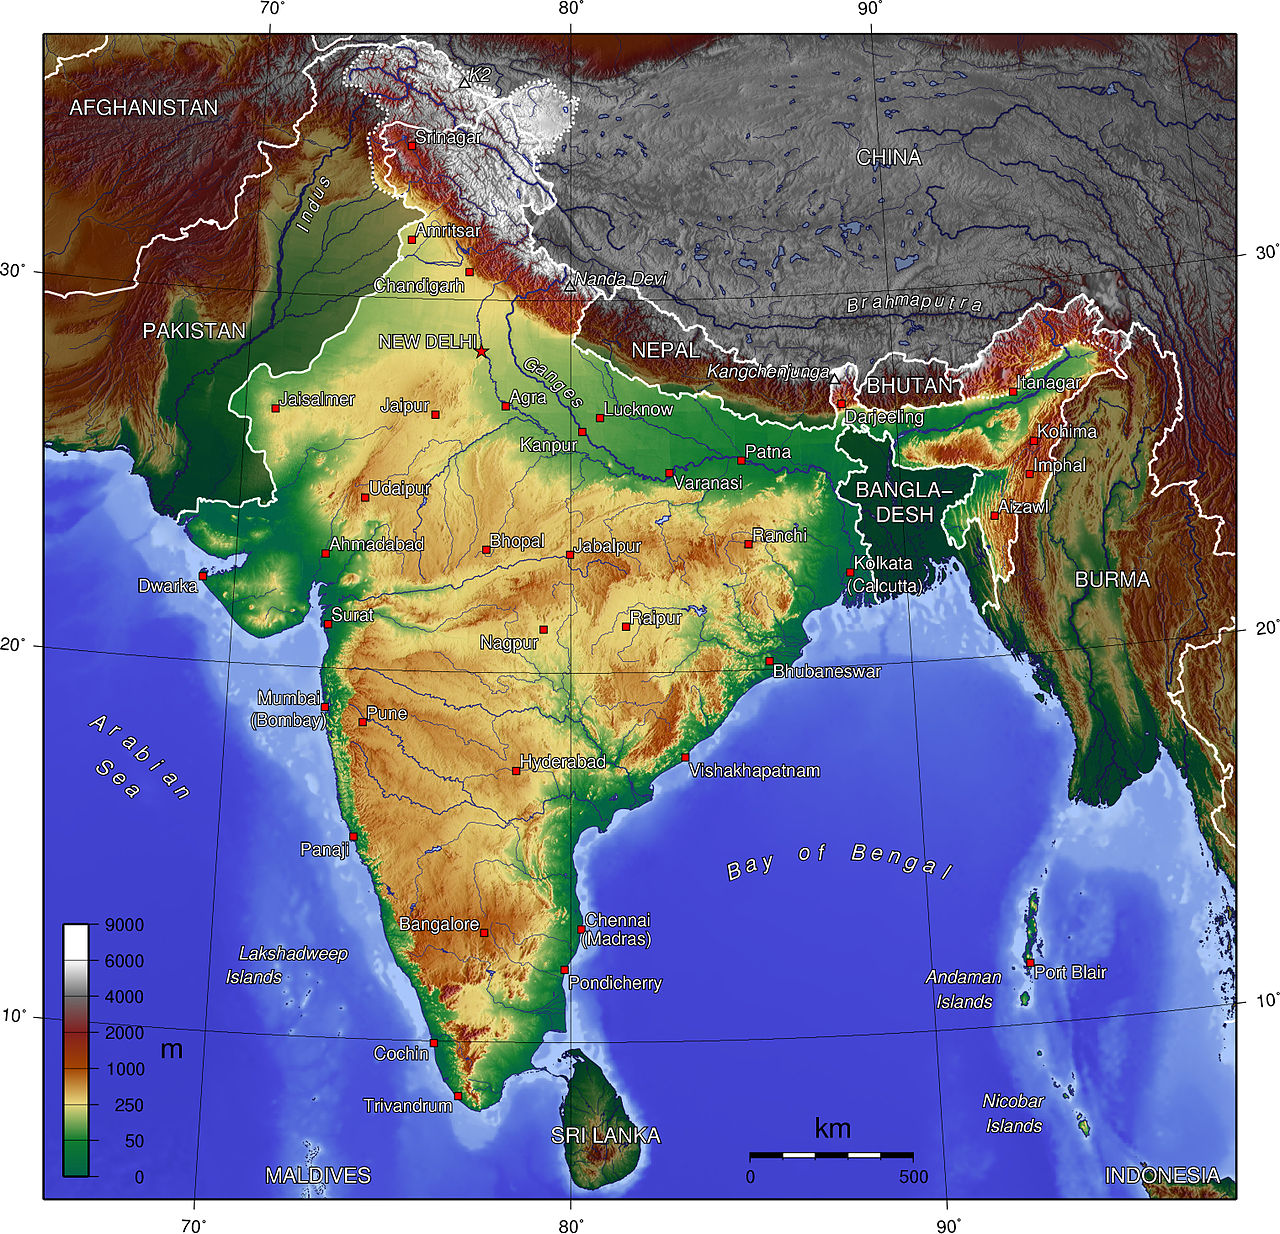
\includegraphics[width=\linewidth]{../images/Elevation-map-of-India.jpg}
% 		\end{figure}
% 		{\tiny \textbf{Fig.\ 21:} Elevation map of India.
% 		Source: Wikimedia Commons - India topo.\\
% 		Eastern Ghats: 600–1600 m (Tracks 1, 4 path).
% 		Indo-Gangetic Plain: $<$200 m (Tracks 2, 3, 5, 6 path).}
% 	\end{columns}
%
% 	\vspace{0.1cm}
% 	\footnotesize
% 	\textbf{Orographic disruption of feedback:}
% 	Steep slopes ($>$8$^\circ$) increase drainage 2–3$\times$ vs.\ flat terrain $\to$
% 	no infiltration $\to$ soil stays dry $\to$ LHF collapses $\to$ MD decays.
% 	\footnotesize \textit{Plains tracks survive 2× longer
% 		(mean 135h) than Eastern Ghats tracks (mean 77h).}
% \end{frame}
%
% % -------------------------------------------------------------------
% \setLayout{plain}
% \begin{frame}{Soil Type Control - Clay vs.\ Sandy Soils}
% 	\vspace{-0.5cm}
% 	\begin{columns}[T]
% 		\column{0.49\textwidth}
% 		\begin{figure}
% 			\includegraphics[width=1.05\linewidth]{../../version26-with-ocean-masking-lsm/output_2024/MD_track_2024.png}
% 		\end{figure}
%
% 		\column{0.49\textwidth}
% 		\begin{figure}
% 			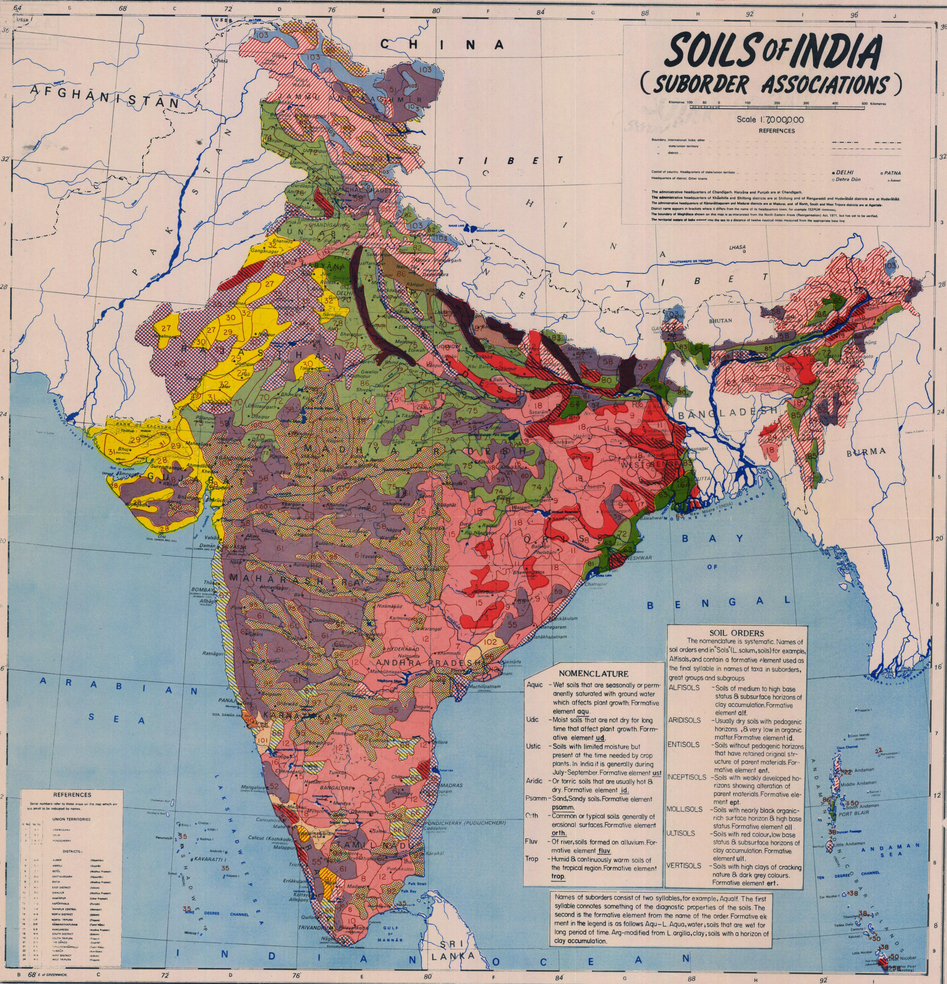
\includegraphics[width=0.9\linewidth]{../images/Soiltype-map-of-India.png}
% 		\end{figure}
% 		{\tiny \textbf{Fig.\ 22:} Soil type map of India.
% 		Source: European Soil Data Centre (ESDAC).}
% 	\end{columns}
%
% 	\vspace{0.1cm}
% 	\footnotesize
% 	\begin{tabular}{lcccc}
% 		\toprule
% 		\rowcolor{MyBlue!15}
% 		\textbf{Region}        & \textbf{Soil Type}         & \textbf{Tracks} &
% 		\textbf{Mean Duration} & \textbf{Typical FSI}                                          \\
% 		\midrule
% 		Eastern coastal belt   & Sandy-loam, lateritic      & T1, T4          & 77 h  & $<$0.1 \\
% 		Indo-Gangetic Plain    & Clay-rich (high retention) & T2, T3, T5, T6  & 134 h & $>$0.2 \\
% 		\bottomrule
% 	\end{tabular}
% \end{frame}
%
% % -------------------------------------------------------------------
% \section{Hypothesis}
% \setLayout{mainpoint}
% \begin{frame}{}
% 	\frametitle{HYPOTHESIS TESTING}
% \end{frame}
%
% % -------------------------------------------------------------------
% \setLayout{horizontal}
% \begin{frame}{H1 \& H2 - FSI Determines Longevity, Diurnal Coupling Sustains It}
% 	\begin{columns}
% 		\column{0.50\textwidth}
% 		\begin{block}{\small H1 - Coupling Strength (FSI)}
% 			\footnotesize
% 			\textbf{Claim:} FSI $>$ 0.4 $\to$ long-lived; FSI $<$ 0.1 $\to$ short-lived.
% 			\vspace{0.2cm}
% 			\begin{tabular}{lcc}
% 				\toprule
% 				\rowcolor{MyBlue!15}
% 				Category            & FSI range & Mean duration \\
% 				\midrule
% 				Strong (T2, T3, T6) & 0.40–0.64 & 123 h         \\
% 				Moderate (T5)       & 0.21      & 165 h$^*$     \\
% 				Weak (T1, T4)       & 0.03–0.06 & 77 h          \\
% 				\bottomrule
% 			\end{tabular}
% 			\vspace{0.1cm}
% 			{\tiny $^*$Track 5 anomaly: memory compensates.}
% 			\vspace{0.1cm}
%
% 			\textbf{Verdict: \textcolor{DarkGreen}{\ding{51} Supported}}
% 			(with Track 5 as instructive exception).
% 		\end{block}
%
% 		\column{0.50\textwidth}
% 		\begin{block}{\small H2 - Diurnal Land Coupling}
% 			\footnotesize
% 			\textbf{Claim:} Land-phase diurnal SHF amplitude is $4\times$ ocean.
% 			\vspace{0.2cm}
% 			\begin{tabular}{lcc}
% 				\toprule
% 				\rowcolor{MyBlue!15}
% 				Phase          & SHF amplitude                                     & $\Delta$SHF      \\
% 				\midrule
% 				Ocean          & 13.54 W/m$^2$                                     & $-$11.66 W/m$^2$ \\
% 				Land           & 77.57 W/m$^2$                                     & $+$4.45 W/m$^2$  \\
% 				\midrule
% 				\textbf{Ratio} & \multicolumn{2}{c}{\textbf{5.7$\times$ stronger}}                    \\
% 				\bottomrule
% 			\end{tabular}
%
% 			\vspace{0.2cm}
% 			\textbf{Verdict: \textcolor{DarkGreen}{\ding{51} Supported}}
% 			Diurnal amplitude change ($\sim$47 W/m$^2$) is
% 			consistent across all Ocean-to-Land tracks.
% 		\end{block}
% 	\end{columns}
% \end{frame}
%
% % -------------------------------------------------------------------
% \setLayout{horizontal}
% \begin{frame}{H3 \& H4 - Antecedent Moisture, Heat Flux Transition at Landfall}
% 	\begin{columns}
% 		\column{0.50\textwidth}
% 		\begin{block}{\small H3 - ASM Predicts FSI}
% 			\footnotesize
% 			\textbf{Claim:} ASM strongly predicts FSI ($r \approx 0.92$).
%
% 			\textbf{Result:} $r = 0.921$ - 95\% of FSI variance
% 			explained by pre-monsoon soil moisture. \\
% 			Wet soil $\to$ greater moisture availability $\to$
% 			enhanced ET $\to$ stronger LHF $\to$ higher FSI.
%
% 			\vspace{0.2cm}
% 			\textbf{Verdict: \textcolor{DarkGreen}{\ding{51} Strongly Supported}}
% 		\end{block}
%
% 		\column{0.50\textwidth}
% 		\begin{block}{\small H4 - Landfall Heat Flux Transition}
% 			\footnotesize
% 			\textbf{Ocean-to-Land (T1, T4, T5) - pre vs.\ post landfall:}
% 			\begin{tabular}{lccc}
% 				\toprule
% 				\rowcolor{MyBlue!15}
% 				Track & $\Delta$LHF & $\Delta$SHF & $\Delta$Total \\
% 				\midrule
% 				T1    & $+$36       & $+$5.8      & $+$42 W/m$^2$ \\
% 				T4    & $+$58       & $+$6.4      & $+$65 W/m$^2$ \\
% 				T5    & $+$54       & $+$16.5     & $+$70 W/m$^2$ \\
% 				\bottomrule
% 			\end{tabular}
% 			\vspace{0.1cm}
%
% 			LHF retention post-landfall $>$60\% of oceanic supply -
% 			confirms Brown Ocean Effect. SHF reversal (Track 5: $+$4.3 W/m$^2$)
% 			= land surface actively heating MD.
%
% 			\textbf{Verdict: \textcolor{DarkGreen}{\ding{51} Supported}}
% 		\end{block}
% 	\end{columns}
% \end{frame}
%
% % -------------------------------------------------------------------
% \setLayout{horizontal}
% \begin{frame}{H5 \& H6 - Soil Type, TSI, and Antecedent Moisture as Precondition}
% 	\begin{columns}
% 		\column{0.50\textwidth}
% 		\begin{block}{\small H5 - Soil Type Sets the Stage}
% 			\footnotesize
% 			\textbf{Clay (IGP) vs.\ Sand (Coastal):}
% 			\begin{itemize}
% 				\item Clay (T2, T3, T6): $\beta = 0.10$, high retention
% 				      $\to$ FSI $>$ 0.4, duration $>$100 h
% 				\item Sandy-loam (T1, T4): $\beta = 0.35$,
% 				      rapid runoff $\to$ FSI $<$ 0.1, duration $<$80 h
% 			\end{itemize}
% 			\textbf{Mean TSI = 0.39}: terrain explains 39\% of variance.
% 			TSI range: 0.18 (T4) to 0.71 (T3) - large track-to-track spread.
%
% 			\textbf{Verdict: \textcolor{DarkGreen}{\ding{51} Supported}}
% 		\end{block}
%
% 		\column{0.50\textwidth}
% 		\begin{block}{\small H6 - High ASM Necessary but Not Sufficient}
% 			\footnotesize
% 			\textbf{Claim:} High ASM ($>$0.3) provides fuel, but without
% 			clay soil + FSI $>$ 0.4 + ACF $>$ 0.3, even wet soils cannot
% 			sustain the MD.
%
% 			\vspace{0.1cm}
% 			\textbf{Track 5 evidence:} ASM = 0.319 (moderate-wet) $+$
% 			ACF = 0.525 (strong memory) $+$ moderate FSI
% 			$\to$ survived 165 h via memory buffer, \textit{not}
% 			coupling efficiency.
%
% 			\vspace{0.1cm}
% 			Three conditions needed simultaneously:
% 			\begin{enumerate}
% 				\item Clay soil texture
% 				\item FSI $>$ 0.4 (active coupling)
% 				\item ACF $>$ 0.3 (soil memory)
% 			\end{enumerate}
%
% 			\textbf{Verdict: \textcolor{DarkGreen}{\ding{51} Supported}}
% 		\end{block}
% 	\end{columns}
% \end{frame}
%
% % -------------------------------------------------------------------
% \section{Conclusions}
% \setLayout{mainpoint}
% \begin{frame}{}
% 	\frametitle{CONCLUSIONS}
% \end{frame}
%
% % -------------------------------------------------------------------
% \setLayout{vertical}
% \begin{frame}{Conclusions - Monsoon Depression Inland Longevity}
% 	\vspace{-0.2cm}
% 	\footnotesize
% 	\centering
% 	\begin{adjustbox}{width=\textwidth,center}
% 		\begin{tabular}{p{2.8cm} p{4.5cm} p{5.2cm}}
% 			\toprule
% 			\rowcolor{MyBlue!15}
% 			\textbf{Hypothesis}              & \textbf{Finding}                                                      & \textbf{Physical Interpretation}                          \\
% 			\midrule
% 			H1: FSI determines longevity     & FSI $>$0.4 $\to$ $\geq$100h (4 of 5 tracks)                           & Strong TP–SWVL1 coupling sustains the vortex core         \\
% 			H2: Diurnal coupling             & Land SHF amplitude 5.7$\times$ ocean; $\Delta$SHF $\approx$47 W/m$^2$ & Daytime heating + nighttime LHF = pulsing energy cycle    \\
% 			H3: ASM predicts FSI             & $r = 0.921$ (very strong)                                             & Wetter pre-monsoon soil $\to$ stronger coupling during MD \\
% 			H4: Landfall transition          & LHF retention $>$60\%; SHF reversal                                   & Brown Ocean replaces ocean moisture at landfall           \\
% 			H5: Soil type                    & Clay (IGP) 134h vs.\ Sand 77h (mean)                                  & Clay retains moisture; sand drains before feedback forms  \\
% 			H6: ASM necessary not sufficient & Three conditions needed simultaneously                                & Memory + coupling + soil type all required                \\
% 			\bottomrule
% 		\end{tabular}
% 	\end{adjustbox}
%
% 	\vspace{0.2cm}
% 	\begin{block}{\small Overall Conclusion}
% 		\footnotesize
% 		\textbf{MD longevity is governed by two distinct but complementary modes:}
% 		\begin{enumerate}
% 			\item \textbf{Efficiency Mode} (Tracks 2, 3, 6): High CE driven by clay soils
% 			      and strong TP–SWVL1 coupling directly fuels the low-pressure system.
% 			\item \textbf{Memory Mode} (Track 5): High soil moisture persistence (ACF)
% 			      acts as a ``buffer'' - sustaining the system even with moderate coupling.
% 		\end{enumerate}
% 		Tracks failing to reach clay-rich terrain and forming over coastal/Eastern Ghats
% 		sandy soils (T1, T4) lack both modes and decay within 80 h.
% 	\end{block}
% \end{frame}
%
% % -------------------------------------------------------------------
% \setLayout{horizontal}
% \begin{frame}{Limitations \& Future Work}
% 	\begin{columns}
% 		\column{0.50\textwidth}
% 		\begin{block}{\small Current Limitations}
% 			\footnotesize
% 			\begin{itemize}
% 				\item \textbf{Sample size:} 6 tracks (1 season, 2024). Statistical
% 				      power is limited; multi-year analysis needed.
% 				\item \textbf{ERA5 resolution:} 28 km smooths soil heterogeneity;
% 				      coastal SWVL1 may be underestimated.
% 				\item \textbf{Causality:} TP–SWVL1 correlation cannot confirm
% 				      direction (Granger test failed due to short track length
% 				      100–140 h).
% 				\item \textbf{HWSD integration:} Clay content estimated from track
% 				      region; direct soil texture mapping pending.
% 				\item \textbf{SST effects:} Late-season track differences may
% 				      partly reflect SST gradient changes, not only soil.
% 			\end{itemize}
% 		\end{block}
%
% 		\column{0.50\textwidth}
% 		\begin{block}{\small Recommended Future Work}
% 			\footnotesize
% 			\begin{itemize}
% 				\item Multi-year validation (2022–2025) to test
% 				      FSI $>$ 0.4 threshold robustness.
% 				\item Granger causality with longer tracks or reanalysis composites.
% 				\item HWSD clay content along each track (soilgrids.org integration).
% 				\item Post-landfall TSI in 24h windows to resolve temporal evolution
% 				      of terrain effect.
% 				\item Diurnal LHF composite (pre vs.\ post landfall, by hour-of-day).
% 				\item FSI/CE as predictive metrics for operational MD duration
% 				      forecasting (target $R^2 > 0.75$).
% 				\item 850 hPa vorticity analysis alongside 10m fields.
% 			\end{itemize}
% 		\end{block}
% 	\end{columns}
% \end{frame}

% -------------------------------------------------------------------
\section{References}
\setLayout{vertical}
\begin{frame}[allowframebreaks]{References}
	\frametitle{References}
	\nocite{*}
	\scriptsize
	\printbibliography
\end{frame}

% -------------------------------------------------------------------
\section{End}
\setLayout{blank}
\begin{frame}
	\centering
	\vspace{3.5cm}
	\textbf{\Huge Thank You} \\
	\vspace{1cm}
	\textbf{Questions and Suggestions}
\end{frame}

\end{document}
